%%
%% This is file `sample-sigconf-authordraft.tex',
%% generated with the docstrip utility.
%%
%% The original source files were:
%%
%% samples.dtx  (with options: `all,proceedings,bibtex,authordraft')
%% 
%% IMPORTANT NOTICE:
%% 
%% For the copyright see the source file.
%% 
%% Any modified versions of this file must be renamed
%% with new filenames distinct from sample-sigconf-authordraft.tex.
%% 
%% For distribution of the original source see the terms
%% for copying and modification in the file samples.dtx.
%% 
%% This generated file may be distributed as long as the
%% original source files, as listed above, are part of the
%% same distribution. (The sources need not necessarily be
%% in the same archive or directory.)
%%
%%
%% Commands for TeXCount
%TC:macro \cite [option:text,text]
%TC:macro \citep [option:text,text]
%TC:macro \citet [option:text,text]
%TC:envir table 0 1
%TC:envir table* 0 1
%TC:envir tabular [ignore] word
%TC:envir displaymath 0 word
%TC:envir math 0 word
%TC:envir comment 0 0
%%
%% The first command in your LaTeX source must be the \documentclass
%% command.
%%
%% For submission and review of your manuscript please change the
%% command to \documentclass[manuscript, screen, review]{acmart}.
%%
%% When submitting camera ready or to TAPS, please change the command
%% to \documentclass[sigconf]{acmart} or whichever template is required
%% for your publication.
%%
%%
\documentclass[sigconf]{acmart}


\usepackage{amsmath,amsfonts}
\usepackage{algorithm}
\usepackage{graphicx}
%\usepackage{textcomp}
%\usepackage{xcolor}
\usepackage{array}            % ← 必须：提供 \newcolumntype
\usepackage{subfig}           % 建议: \usepackage[caption=false,font=footnotesize]{subfig}
\usepackage{algpseudocode}
\usepackage{makecell}
\usepackage{multirow}
\usepackage{tikz}
%%
%% \BibTeX command to typeset BibTeX logo in the docs
\AtBeginDocument{%
  \providecommand\BibTeX{{%
    Bib\TeX}}}

\definecolor{myyellow}{RGB}{255,217,101}
\definecolor{myblue}{RGB}{102,153,255}
\definecolor{mygreen}{RGB}{146,208,80}

% ---- 实用宏 ----
\newcommand*\circled[1]{%
  \tikz[baseline=(char.base)]{
    \node[text=white, circle, draw, fill=black, inner sep=0.3pt] (char) {#1};}}
\newcommand*\circledy[1]{%
  \tikz[baseline=(char.base)]{
    \node[text=black, circle, draw, fill=myyellow, inner sep=0.3pt] (char) {#1};}}
\newcommand*\circledb[1]{%
  \tikz[baseline=(char.base)]{
    \node[text=black, circle, draw, fill=myblue, inner sep=0.3pt] (char) {#1};}}
\newcommand*\circledg[1]{%
  \tikz[baseline=(char.base)]{
    \node[text=black, circle, draw, fill=mygreen, inner sep=0.3pt] (char) {#1};}}



%% Rights management information.  This information is sent to you
%% when you complete the rights form.  These commands have SAMPLE
%% values in them; it is your responsibility as an author to replace
%% the commands and values with those provided to you when you
%% complete the rights form.
\setcopyright{acmlicensed}
\copyrightyear{2026}
\acmYear{2026}
\acmDOI{XXXXXXX.XXXXXXX}
%% These commands are for a PROCEEDINGS abstract or paper.
\acmConference[ICS'26]{July 06--09,
  2026}{Belfast, Northern Ireland, UK}
%%
%%  Uncomment \acmBooktitle if the title of the proceedings is different
%%  from "Proceedings of ...''!
%%
%%\acmBooktitle{Woodstock '18: ACM Symposium on Neural Gaze Detection,
%%  June 03--05, 2018, Woodstock, NY}
%\acmISBN{978-1-4503-XXXX-X/2018/06}


%%
%% Submission ID.
%% Use this when submitting an article to a sponsored event. You'll
%% receive a unique submission ID from the organizers
%% of the event, and this ID should be used as the parameter to this command.
%%\acmSubmissionID{123-A56-BU3}

%%
%% For managing citations, it is recommended to use bibliography
%% files in BibTeX format.
%%
%% You can then either use BibTeX with the ACM-Reference-Format style,
%% or BibLaTeX with the acmnumeric or acmauthoryear sytles, that include
%% support for advanced citation of software artefact from the
%% biblatex-software package, also separately available on CTAN.
%%
%% Look at the sample-*-biblatex.tex files for templates showcasing
%% the biblatex styles.
%%

%%
%% The majority of ACM publications use numbered citations and
%% references.  The command \citestyle{authoryear} switches to the
%% "author year" style.
%%
%% If you are preparing content for an event
%% sponsored by ACM SIGGRAPH, you must use the "author year" style of
%% citations and references.
%% Uncommenting
%% the next command will enable that style.
%%\citestyle{acmauthoryear}


%%
%% end of the preamble, start of the body of the document source.
\begin{document}

%%
%% The "title" command has an optional parameter,
%% allowing the author to define a "short title" to be used in page headers.
\title{Accelerating Multi-Scale Deformable Attention Using Near-Memory-Processing Architecture}

%%
%% The "author" command and its associated commands are used to define
%% the authors and their affiliations.
%% Of note is the shared affiliation of the first two authors, and the
%% "authornote" and "authornotemark" commands
%% used to denote shared contribution to the research.
\author{Huize Li}
%\authornote{Both authors contributed equally to this research.}
%\orcid{1234-5678-9012}
%\author{G.K.M. Tobin}
%\authornotemark[1]
%\email{webmaster@marysville-ohio.com}
\affiliation{%
  \institution{University of Central Florida}
  \city{Orlando}
  \state{Florida}
  \country{USA}
}
\email{huize.li@ucf.edu}

\author{Qinggang Wang}
\affiliation{%
  \institution{Huazhong University of Sci. \& Tech.}
  \city{Wuhan}
  \country{China}}
\email{qgwang@hust.edu.cn}

\author{Bin Gao}
\affiliation{%
  \institution{National University of Singapore}
  \city{Singapore}
  \country{Singapore}
}
\email{bingao@comp.nus.edu.sg}

\author{Dan Chen}
\affiliation{%
  \institution{National University of Singapore}
  \city{Singapore}
  \country{Singapore}
}
\email{danchen@nus.edu.sg}


\author{Yu Huang}
\affiliation{%
  \institution{Huazhong University of Sci. \& Tech.}
  \city{Wuhan}
  \country{China}}
\email{yuh@hust.edu.cn}

\author{Xin Xin}
\authornote{Corresponding author is Xin Xin.}
%\orcid{1234-5678-9012}
%\author{G.K.M. Tobin}
%\authornotemark[1]
%\email{webmaster@marysville-ohio.com}
\affiliation{%
  \institution{University of Central Florida}
  \city{Orlando}
  \state{Florida}
  \country{USA}
}
\email{xin.xin@ucf.edu}


%%
%% The abstract is a short summary of the work to be presented in the
%% article.
\begin{abstract}
Multi-Scale Deformable Attention (MSDAttn) has become a fundamental component in various vision tasks due to its effective multi-scale grid sampling (MSGS). However, its reliance on random sampling results in highly irregular memory access patterns, making it a memory-intensive operation inefficient for GPUs. Near-memory processing (NMP) offers a promising solution for accelerating memory-bound kernels, yet existing NMP-based attention accelerators remain suboptimal for MSDAttn due to incompatible load balancing and data reuse strategies. Specifically, current NMP solutions uniformly distribute processing elements (PEs) across all banks, leading to significant PE underutilization and excessive cross-bank data transfers. Moreover, most rely on locality-based reuse, which fails under MSDAttn’s unpredictable sampling patterns.

To address these challenges, this paper presents \textit{DANMP}, a hardware–software co-designed NMP-based MSDAttn accelerator. On the hardware side, \textit{DANMP} adopts non-uniform NMP integration to handle unbalanced workloads, allocating PEs only in select banks for hot entries, while cold data are processed at the bank-group level—reducing PE idleness and cross-bank transfers. On the software side, it introduces a clustering-and-packing (CAP) method that leverages clustering to improve temporal locality in query processing, enhancing data reuse. Finally, we implement host–NMP co-optimization techniques, including an optimized programming model, customized instructions, and a tailored dataflow. Experiments on object detection inference show that \textit{DANMP} achieves 97.43$\times$ speedup and 208.47$\times$ energy efficiency improvement over NVIDIA A6000 GPU.

\end{abstract}

%%
%% The code below is generated by the tool at http://dl.acm.org/ccs.cfm.
%% Please copy and paste the code instead of the example below.
\begin{CCSXML}
<ccs2012>
   <concept>
       <concept_id>10010520.10010521.10010542.10010294</concept_id>
       <concept_desc>Computer systems organization~Neural networks</concept_desc>
       <concept_significance>500</concept_significance>
       </concept>
 </ccs2012>
\end{CCSXML}

\ccsdesc[500]{Computer systems organization~Neural networks}

\keywords{Hardware Accelerators, Machine Learning, Memory Systems, In-memory Computing}

%%
%% This command processes the author and affiliation and title
%% information and builds the first part of the formatted document.
\maketitle

\section{Introduction}

The \textit{Detection Transformer} (DETR)~\cite{carion2020end, gupta2022ow, beal2020toward, Fang2021} has recently achieved remarkable success in object detection by combining \textit{convolutional neural networks} (CNNs) with a Transformer-based encoder-decoder architecture~\cite{Vaswani17}. Despite its improvement in accuracy, DETR suffers from slow convergence, requiring significantly more training epochs than conventional object detection methods~\cite{du2018understanding, xie2021oriented, chen2016r}. {To address this limitation, \textit{multi-scale deformable attention} (MSDAttn/MSDeformAttn) has been introduced, effectively reducing training/inference costs and computational complexity.} Inspired by deformable convolution~\cite{Dai2017ICCV}, MSDAttn selectively attends to a sparse set of reference points across multi-scale feature maps, avoiding the exhaustive computation inherent in traditional attention mechanisms~\cite{Vaswani17}. By leveraging efficient \textit{multi-scale grid-sampling} (MSGS), MSDAttn achieves state-of-the-art training/inference efficiency. However, the irregular distribution of reference point sampling introduces random memory access overhead, significantly constraining system performance~\cite{xu2024defa}.


Recently, there has been growing interest in hardware-software co-designed solutions to mitigate random memory access overhead. These solutions encompass various platforms, including GPUs~\cite{zhu2021deformable, longformer20, Tay20, Rajpurkar18}, \textit{Field Programmable Gate Arrays} (FPGAs)~\cite{Zhang21fpga, Fan2022fpga, bai2024dac, Zhang21}, and \textit{Application Specific Integrated Circuits} (ASICs)~\cite{xu2024defa, Qu22, Qin23isca, Lu21}. While these co-designed approaches outperform software-only solutions with hardware-friendly scheduling and computation techniques, they remain compute-centric and are still constrained by off-chip memory bandwidth when accelerating memory-intensive MSDAttn workloads. As a result, they suffer from high-latency off-chip accesses due to the large volume of randomly sampled feature maps~\cite{xu2024defa}. Given the increasing demand for low latency object detection, improving the efficiency of MSDAttn could have a substantial impact on both performance and scalability.

\begin{figure}[t]
\centering
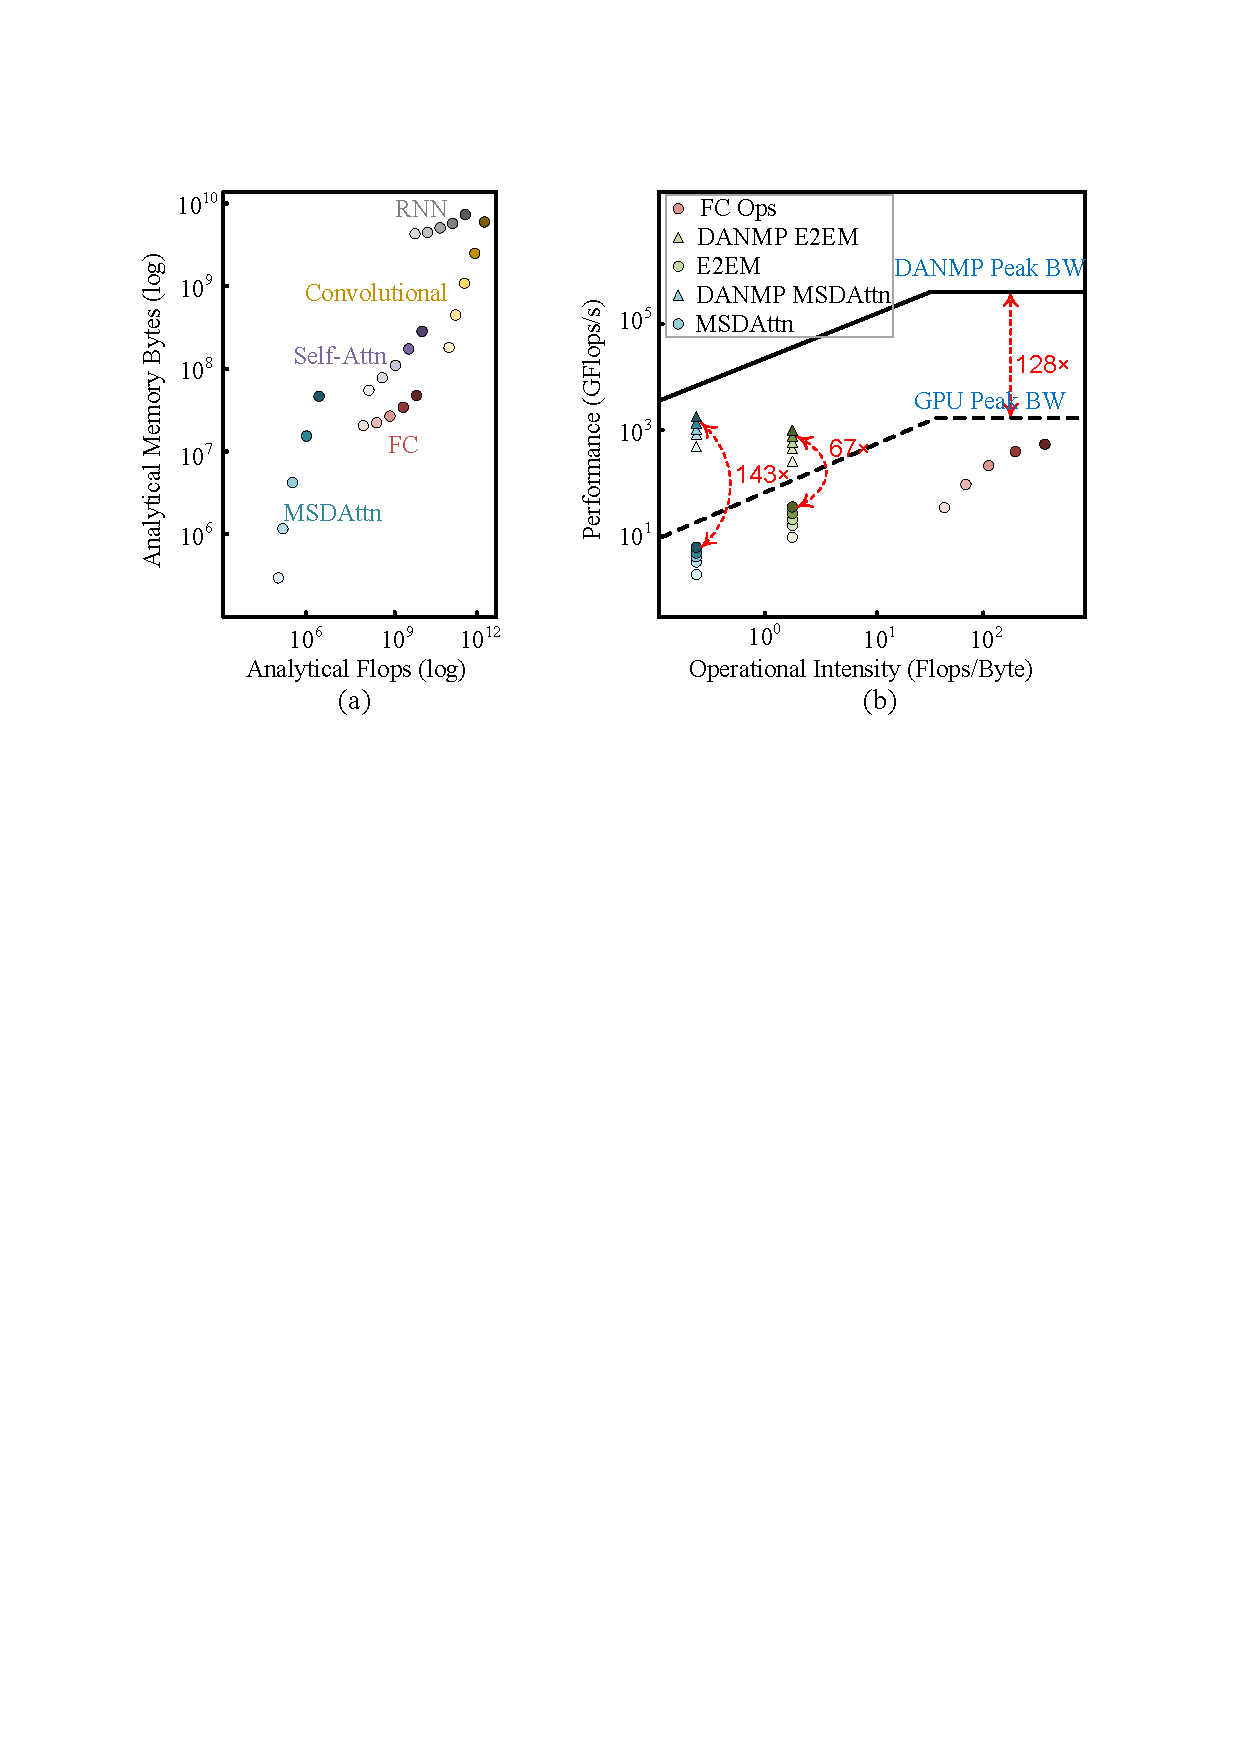
\includegraphics[width=8.3cm]{figures/exp/cmratio.pdf}
\vspace{-1em}
\caption{(a) Computational and memory footprint of common deep learning operators across different batch sizes (darker shades indicate larger batches), (b) {Bandwidth roofline} model showing performance gains, including operator-level speedups for FC and MSDAttn, as well as end-to-end model (E2EM) acceleration enabled by \textit{DANMP}}
\label{cm_ratio}
%\vspace{-2em}
\end{figure}

A quantitative comparison of the computational and memory access requirements for various neural network operations is presented in Figure~\ref{cm_ratio}(a) ({The experimental configuration is same to Section~\ref{motivation_ana}}). Unlike \textit{recurrent neural networks} (RNNs), convolutions, \textit{full-connection} (FC), and \textit{self-attention} (Self-Attn) operations, {MSDAttn exhibits exceptionally low operational intensity---less than 10\% of the compute–bandwidth intersection in the Roofline model---indicating that its performance is primarily constrained by memory bandwidth rather than arithmetic throughput. This memory-bound behavior arises mainly from multi-scale grid sampling (\circled{2} in Figure~\ref{msattention}) and feature aggregation (\circled{3} in Figure~\ref{msattention}).}

Compared to standard self-attention, MSDAttn faces three major challenges.
Irregular Sampling: Sparse and non-uniform sampling across large feature maps leads to unpredictable memory accesses, making prefetching and dataflow optimizations ineffective.
Limited Data Reuse: Hundreds of detection queries target different spatial regions, offering little locality across queries.
Irregular Sparsity and Load Imbalance: MSDAttn prunes data-dependent feature points, creating highly unstructured sparsity and severe load imbalance.
{Unlike previous sparsity accelerators (e.g., SCNN~\cite{parashar2017scnn}, CANDLES~\cite{gudaparthi2022candles}, AWB-GCN~\cite{geng2020awb}, EnGN~\cite{liang2020engn}) that exploit predictable zero patterns, MSDAttn’s query-specific sparsity varies across scales and tokens, breaking regular dataflows and tile reuse. Consequently, its operational intensity remains extremely low, leaving the computation memory-bound.}


This paper presents \textit{DANMP}, the first near-memory processing architecture designed to accelerate MSDAttn in DETR. \textit{DANMP} is a hardware-software co-designed \textit{Dual In-line Memory Module} (DIMM)-based system, built on standard DRAM technology. In contrast to stack-based solutions, which demands specialized 2.5D/3D integration processes such as HBM~\cite{Ahn2015isca, Zhou2022, Ding2023, micro2024li, highp2025} and ReRAM~\cite{ReGNN2022, asadi2024, resqm2020, cpsaa2024, resma2022, splim2025}, the adoption of a DIMM-based NMP~\cite{chen2023, sadimm2025, Kim2022, micro2024ham} enables the use of commodity DDR5 devices and provides large memory capacity (over 64GB) at low cost. By eliminating the off-chip memory bottleneck and exposing higher internal bandwidth, \textit{DANMP} significantly enhances both performance and energy efficiency. Specifically, it raises the {bandwidth roofline} of GPU platform by 128$\times$ in bandwidth-constrained regions (Figure~\ref{cm_ratio}(b)), unlocking optimization opportunities that are infeasible with conventional architectures.


We conducted a detailed characterization of the open-source Deformable DETR (DE-DETR) model~\cite{zhu2021deformable} as a case study (Figure~\ref{cm_ratio} and Figure~\ref{case1}). This analysis quantifies the potential benefits of near-memory processing in accelerating Deformable DETR, specifically highlighting how \textit{DANMP} can optimize performance. In this paper, memory-intensive MSDAttn operations are executed within memory, while compute-intensive FC operations are processed by the host. Additionally, we also performed an NMP-based DETR case study (Figure~\ref{case2}) to identify performance bottlenecks in executing DETR on existing NMP accelerators. Our findings reveal two key challenges that severely limit performance. \textit{PE Idleness Caused by Load Imbalance:} Current NMP solutions often adopt uniform PE integration, leading to idle PEs when mapping irregular MSDAttn workloads. Reassigning tasks to idle PEs introduces significant cross-bank transfers, further increasing memory access overhead. \textit{Bandwidth Wastage Due to Random Memory Access:} Due to the poor data locality in MSDAttn, existing NMP accelerators fail to exploit data reuse efficiently. This leads to underutilization of the ample intra-bank bandwidth and intensifies the pressure on the limited cross-bank bandwidth.


To address these challenges, \textit{DANMP} introduces both hardware and software innovations. On the hardware side, \textit{DANMP} investigates the hierarchical structure of DRAM memory systems and exploits the multi-tiered parallelism across ranks, bank-groups, and banks. Unlike existing NMP architectures, we adopt a non-traditional, uneven integration strategy by implementing PEs only in selected banks. Mapping irregular MSDAttn workloads to the unevenly integrated architecture significantly reduces PE idleness without introducing cross-bank transfers. On the software side, we introduce a \textit{clustering-and-packing} (CAP) method, which significantly enhances data reuse by grouping queries with the same sub-targets. This optimization mitigates random memory access inefficiencies and improves temporal locality. Compared to the GPU platform, \textit{DANMP} achieves 143$\times$ reduction in MSDAttn latency and 67$\times$ improvement in end-to-end DE-DETR inference performance, as shown in Figure~\ref{cm_ratio}(b). This work makes the following key research contributions:

\begin{itemize}
    \item We demonstrate that MSDAttn is constrained by memory bandwidth with our GPU case study. Our NMP-based case study reveals that load imbalance and low data reuse rates are the primary factors behind this constraint.
    \item We introduce \textit{DANMP}, a lightweight DDR5-compatible near-memory processing accelerator designed for MSDAttn execution, achieving 97.43$\times$ performance improvement, 208.47$\times$ energy efficiency improvement against NVIDIA A6000 GPU.
    \item We also explore uneven PE integration, clustering-and-packing algorithm, and host-NMP co-optimizations to enhance the performance of \textit{DANMP}.
\end{itemize}



\begin{figure}[t]
\centering
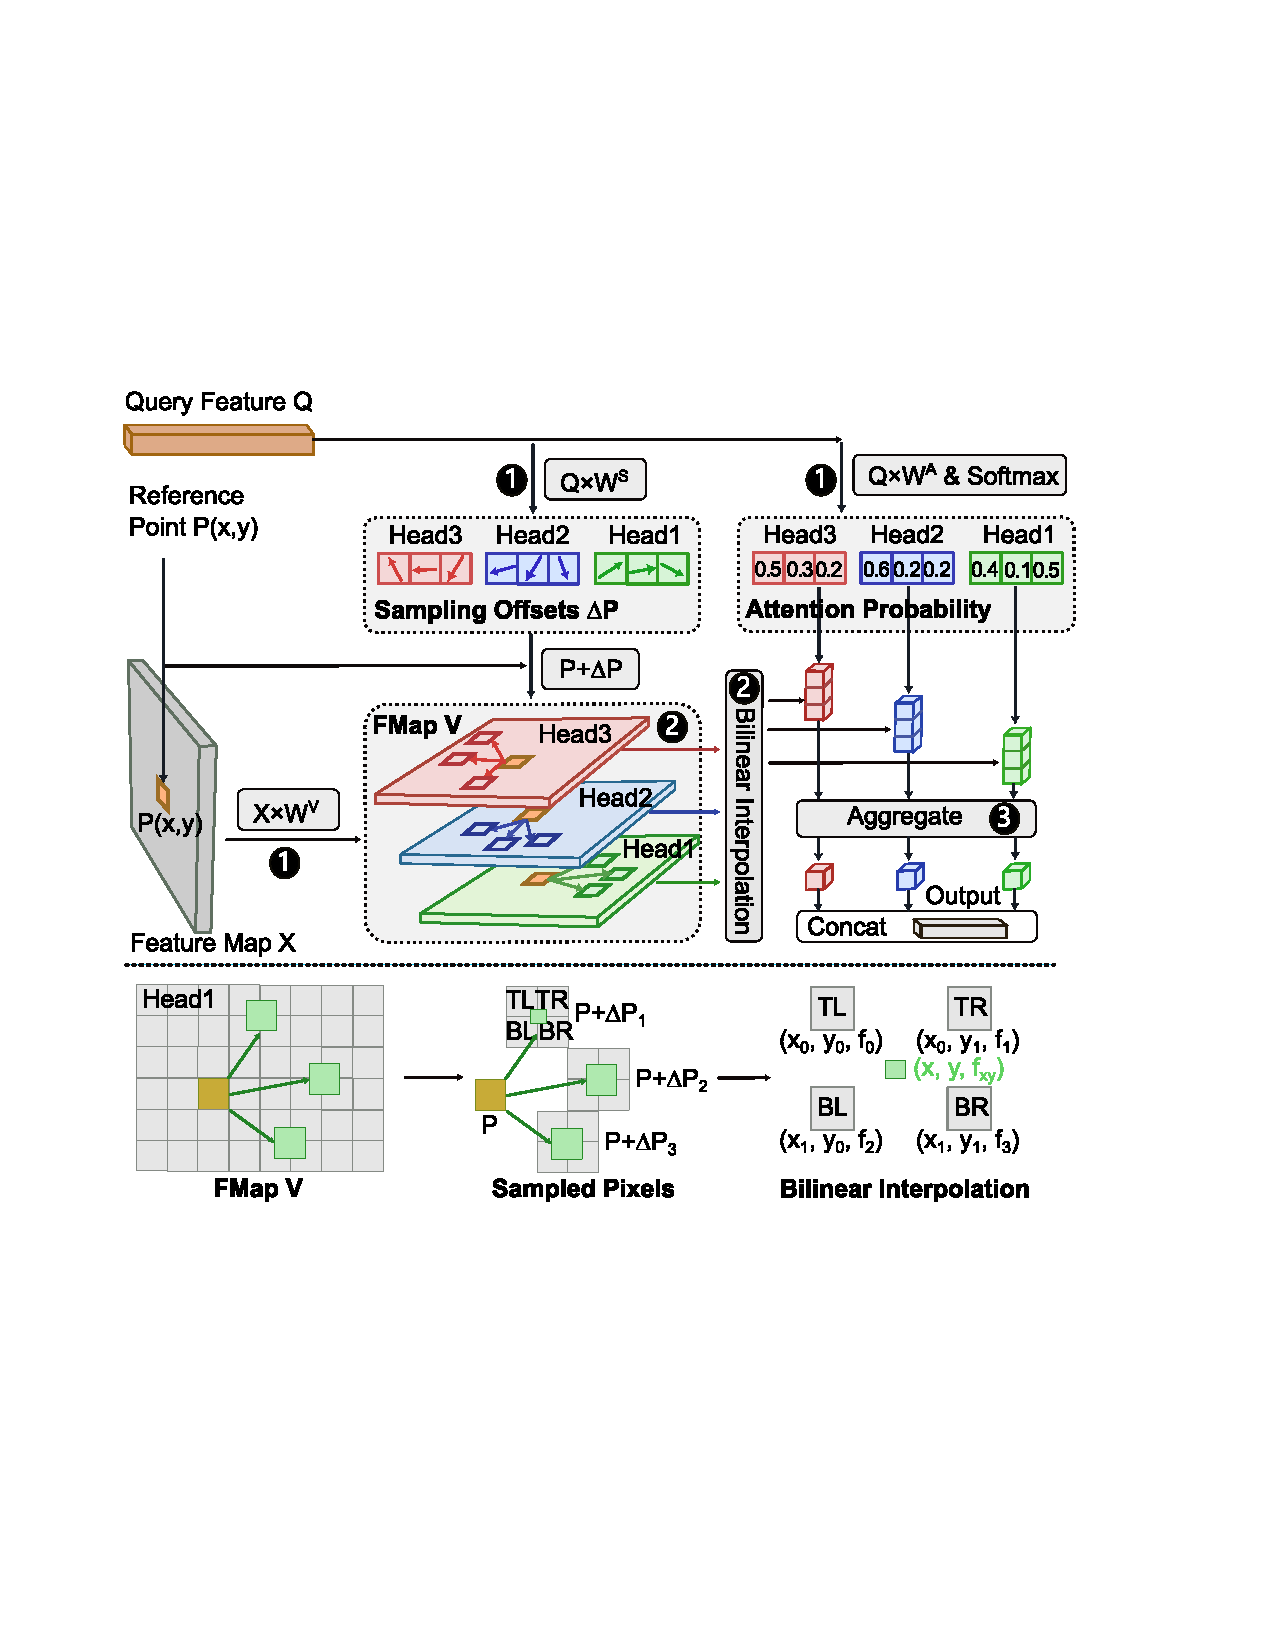
\includegraphics[width=8.3cm]{figures/graph/msattention.pdf}
\vspace{-1em}
\caption{Overview of the MSDAttn}
\label{msattention}
\vspace{-1em}
\end{figure}

\section{Background}
\subsection{Multi-Scale Deformable Attention}
\label{msda}
{
Multi-Scale Deformable Attention (MSDAttn) is a key operation in modern object detectors such as Deformable DETR, where each query dynamically samples a small set of spatial locations across multi-scale feature maps to capture long-range dependencies. 
This data-dependent sampling provides high modeling flexibility but also introduces severe irregularity in memory access, as illustrated in Figure~\ref{msattention}.} MSDAttn identifies relations between each query and a small set of sampling points in multi-scale fmaps $X \in \mathbb{R}^{n\times d}$. Let $n$ and $d$ denote the length of flattened feature maps from $l$ levels ($N = \sum_{i=1}^{l}H_i\times W_i$) and hidden dimension of pixel vectors respectively. Where $H_i$ and $W_i$ denote the height (number of vertical pixels) and width (number of horizontal pixels) of layer $l$. The computation of MSDAttn is calculated by concatenate all $h$ attention heads as equation~(\ref{concat}),

\vspace{-1em}
\begin{equation}
{MSDAttn}(\boldsymbol{Q}, \boldsymbol{P}, \boldsymbol{X}) = Concat(\boldsymbol{H}_1, ... , \boldsymbol{H}_h),
\label{concat}
\end{equation}
the calculation of the output matrix in the $j^{th}$ attention head is shown in equation~(\ref{head_j}),
\begin{equation}
\boldsymbol{H}_j = Softmax(\boldsymbol{Q\cdot W}_j^A) \boldsymbol{\cdot V}_j(\boldsymbol{X},\, {\boldsymbol{P} \oplus \Delta\boldsymbol{P}_j}),
\label{head_j}
\end{equation}
where $\boldsymbol{Q} \in \mathbb{R}^{n\times d}$ and $\boldsymbol{V} = \boldsymbol{X\cdot W}^V \in \mathbb{R}^{n\times d}$ denote the query matrix and the multi-scale fmaps, respectively. $\boldsymbol{P}$ refers to the coordinates of the reference point in each level of fmaps. 
{
$\oplus$ denotes coordinate indexing rather than arithmetic addition, 
i.e., $\boldsymbol{P} \oplus \Delta\boldsymbol{P}_j$ represents sampling locations offset from reference points $\boldsymbol{P}$ by learned displacements $\Delta\boldsymbol{P}_j$. 
$\boldsymbol{V}_j(\boldsymbol{X}, \boldsymbol{P} \oplus \Delta\boldsymbol{P}_j)$ gathers feature values from $\boldsymbol{X}$ via bilinear interpolation at these locations.
$\Delta\boldsymbol{P} = \boldsymbol{Q\cdot W}^S$ denotes the offsets of sampling points. $\boldsymbol{W}^A \in \mathbb{R}^{d\times h\times l\times p}$,}
while $\boldsymbol{W}^V \in \mathbb{R}^{d\times d}$ and $\boldsymbol{W}^S \in \mathbb{R}^{d\times 2n\cdot l\cdot p}$ are learnable weights, where $p$ denotes the fixed number of sampling points in each level of fmaps. {
Although the above equations are expressed in matrix form for compactness, they do not represent dense matrix multiplications. 
Instead, MSDAttn follows a gather–interpolate–accumulate pattern visualized in Figure~\ref{msattention}, which exposes its highly irregular memory behavior.}

%\begin{figure}[t]
%\centering
%\includegraphics[width=8.3cm]{figures/graph/dram.pdf}
%\vspace{-0.5em}
%\caption{Hierarchy architecture of DRAM}
%\label{dram}
%\vspace{-2em}
%\end{figure}

Figure~\ref{msattention} illustrates the visualization process of single-level deformable attention, which is an example of all levels in MSDAttn. The inputs to Deformable DETR include the query feature $Q$, reference point $P(x,y)$, feature map $X$, and all learnable weight matrices. The linear transformations on query $Q$ and feature map $X$ are performed in \circled{1}, involves three fully connected layers (weighted matrix multiplication). Simultaneously, a softmax operation normalizes all points across different levels, which are projected from a row vector of the input query, generating attention probability vectors. In \circled{2}, the \textit{multi-scale grid sampling} (MSGS) procedure applies a \textit{bilinear interpolation} (BI) kernel to process fractional sampling points, retrieving corresponding values from the multi-scale feature maps. In \circled{3}, each pixel vector obtained from sampling is multiplied by an element of the attention probability vector, and all weighted vectors are summed to produce the output of a single attention head. Finally, the outputs from all attention heads are concatenated to generate the final output matrix.



{The bottom of Figure~\ref{msattention} illustrates the MSGS computation. Three sampling points, $P+\Delta P_1$, $P+\Delta P_2$, and $P+\Delta P_3$, are selected on the feature map $V$. Since these points typically lie between discrete pixels, bilinear interpolation is used to estimate their feature values. For a sampling point at $(x, y)$ with interpolated value $f_{xy}$, its four neighboring pixels are: top-left (TL) at $(x_0, y_0)$ with value $f_0$, top-right (TR) at $(x_0, y_1)$ with $f_1$, bottom-left (BL) at $(x_1, y_0)$ with $f_2$, and bottom-right (BR) at $(x_1, y_1)$ with $f_3$. The interpolated value is computed as: $f_{xy} \approx [f_0(x_1-x)(y_1-y)+f_1(x_1-x)(y-y_1)+f_2(x-x_1)(y_1-y)+f_3(x-x_1)(y-y_1)]/[(x_1-x_0)(y_1-y_0)]$. This process involves substantial random memory access due to the irregular distribution of sampling points $P$ and $\Delta P$.}

%{{\bf Comparison with Deformable Convolution.} While both MSDAttn~\cite{zhu2021deformable} and deformable convolution~\cite{Dai2017ICCV} use dynamic, data-dependent sampling, they differ significantly in structure and flexibility. Deformable convolution applies offsets relative to a fixed kernel grid (e.g., $3\times3$) and typically shares them across channels, resulting in constrained, localized sampling with predictable access patterns. In contrast, MSDAttn enables each query to attend to multiple arbitrary positions across the feature map, with sampling determined dynamically per query and per head. It also incorporates multi-scale features and non-local learned sampling, leading to sparse and irregular memory access. These characteristics make MSDAttn far more challenging to accelerate using conventional deformable convolution hardware.}

\begin{figure}[t]
\centering
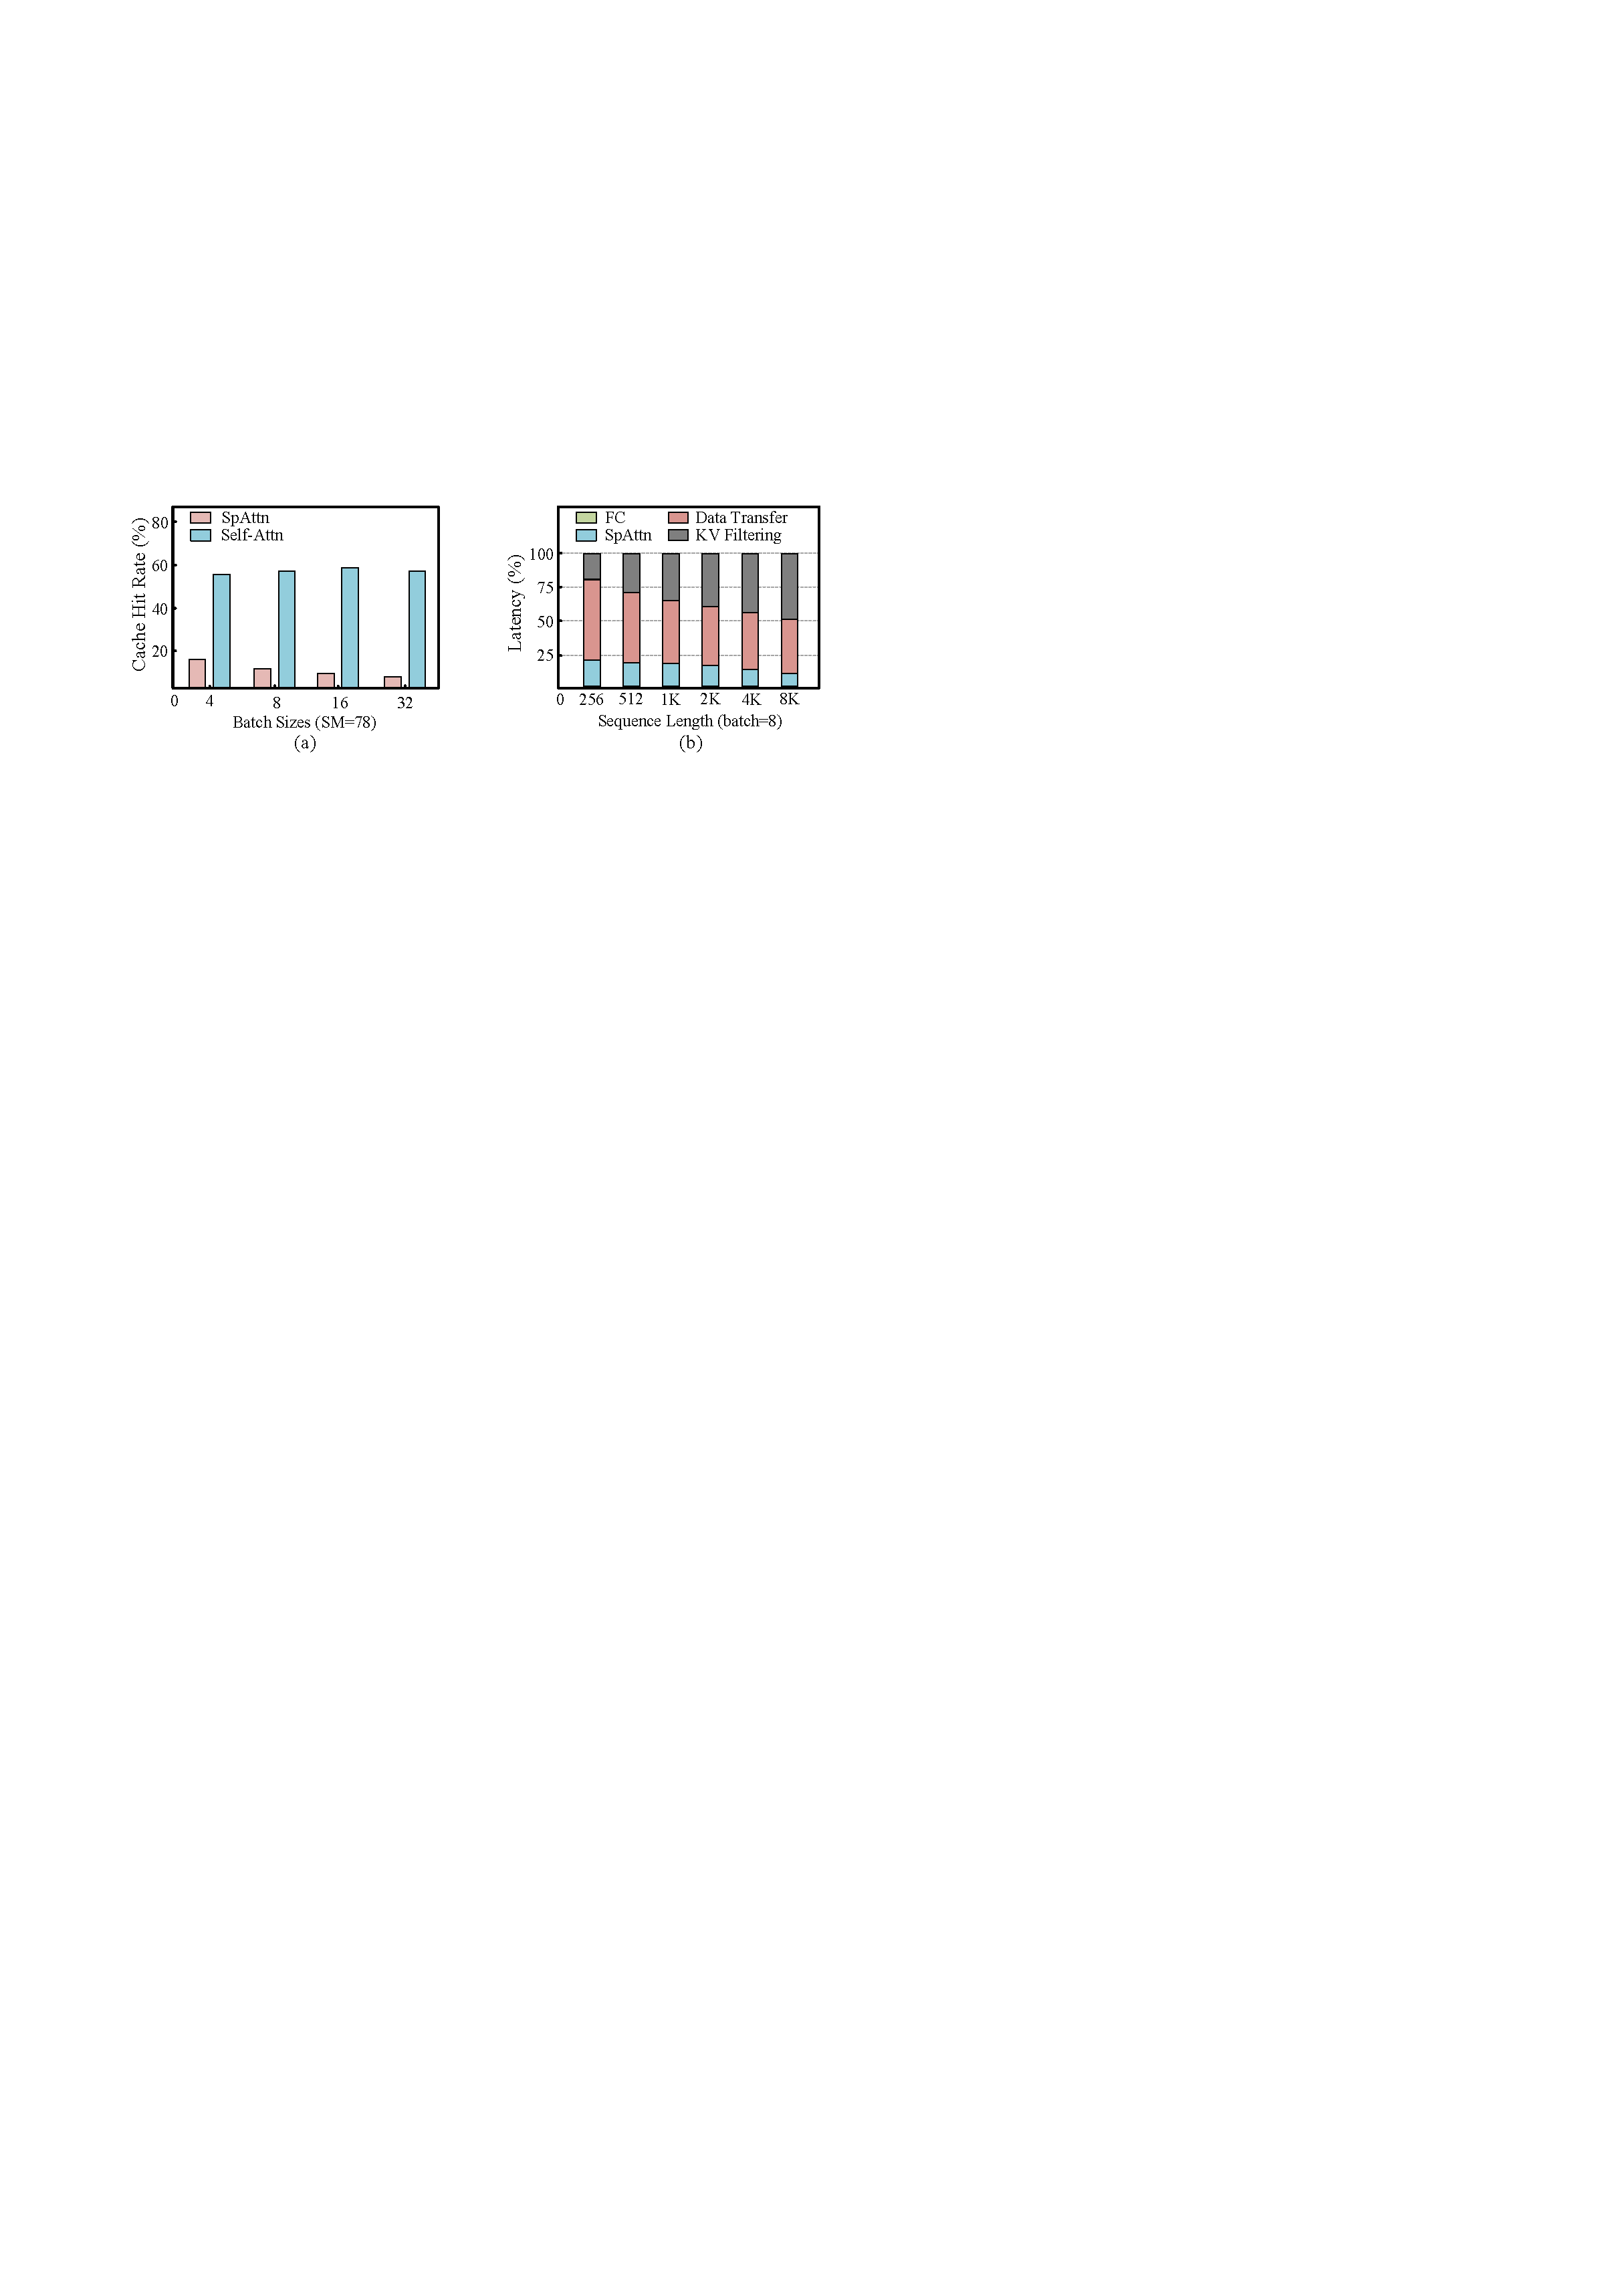
\includegraphics[width=8.39cm]{figures/exp/case1.pdf}
\vspace{-1em}
\caption{(a) Memory bandwidth saturation analysis as the number of \textit{streaming multiprocessors} (SM) increases, (b) Temporal data locality evaluation by varying batch size while keeping cache capacity fixed}
\label{case1}
\vspace{-1em}
\end{figure}

%\subsection{Basics of DRAM}

%As depicted in Figure~\ref{dram}, modern DRAM~\cite{jedec2020} follow a hierarchical structure comprising \textit{channels}, \textit{ranks}, \textit{bank-groups}, and \textit{banks}. At the top level (depth-0), a memory channel includes a host \textit{memory controller} (MC) and multiple DRAM ranks (depth-1) connected to the buffer chip via a data (DQ) path. Each rank consists of eight DRAM chips, configured in an 8-bit lockstep mode to form a 64-bit data bus~\cite{jedec2020}. Within DDR5 DRAM, a single chip is further divided into eight bank-groups (depth-2), with each group containing four banks (depth-3). These banks store data across multiple memory arrays. A uniform \textit{Command/Address} (C/A) signal is sent to all DRAM chips to synchronize their operations. The DQ paths at depth-2 and depth-3 operate similarly to those at depth-1, facilitating data transmission between a rank and its bank-groups as well as between a bank-group and its banks. While individual banks within a DRAM chip can function independently, only one bank can actively access the data paths at depth-1, depth-2, or depth-3 at any given moment.

%Given DRAM’s hierarchical organization, only one rank at a time can utilize the DQ path between the memory controller and ranks. To enhance internal bandwidth, a \textit{processing element} (PE) can be integrated into the buffer chip, allowing the depth-0 path between the MC and buffer chip to remain idle. This setup allows simultaneous data transfers from all ranks to their corresponding PEs, significantly boosting overall bandwidth efficiency. Similarly, placing PEs near bank-groups or individual banks reduces dependency on depth-1 and depth-2 data paths during computations, further optimizing bandwidth performance.



\section{Motivation Analysis}
\label{motivation_ana}
{ The irregular sampling and low locality of MSDAttn make it fundamentally different from standard self-attention. To quantify its inefficiency on existing platforms, we conduct two case studies.}

\subsection{Case Study\#1---Deformable DETR With GPU}
\textbf{Configurations.} To evaluate the benefits of near-memory processing for DETR, we analyze the open-source \textit{Deformable DETR} (DE-DETR) model~\cite{zhu2021deformable} on an NVIDIA RTX A6000 GPU. Our evaluation focuses on object detection inference using the COCO 2017 dataset~\cite{Lin2014}. To assess the impact of data parallelism, we vary the inference batch size from 1 to 32 with darker colors representing larger batch sizes, where 32 is the standard batch size in~\cite{zhu2021deformable}. Memory bandwidth utilization is measured using the \textit{CUDA Profiling Tools Interface} (CUPTI), while \textit{Nsight Compute} (NCU) is employed to analyze L1 and L2 cache hit rates.


\textbf{Bandwidth Roofline Analysis.} We employ the {bandwidth roofline model} provided by \textit{Nsight Compute} (NCU) to illustrate the theoretical performance limits of the GPU platform. Figure~\ref{cm_ratio}(b) presents the {internal bandwidth} data points for the MSDAttn and FC operators. Our analysis reveals distinct computational characteristics for different components of the model, i.e., MSDAttn exhibits low computational intensity but high memory demands, FC is more compute-intensive. The operational intensity of MSDAttn remains low and constant across batch sizes, as it performs a fixed number of grid-sampling operations and corresponding vector-matrix multiplications. In contrast, FC’s operational intensity increases with batch size due to enhanced data reuse, as all queries in the batch share the same learnable weight matrices. Our findings indicate that the \textit{end-to-end model} (E2EM) remains in the memory-bound region, as its operational intensity is primarily determined by the high proportion of MSDAttn ~\cite{xu2024defa}. As batch size increases, both MSDAttn and the full model approach the system’s theoretical performance limits {since bandwidth limitation}.


\begin{figure}[t]
\centering
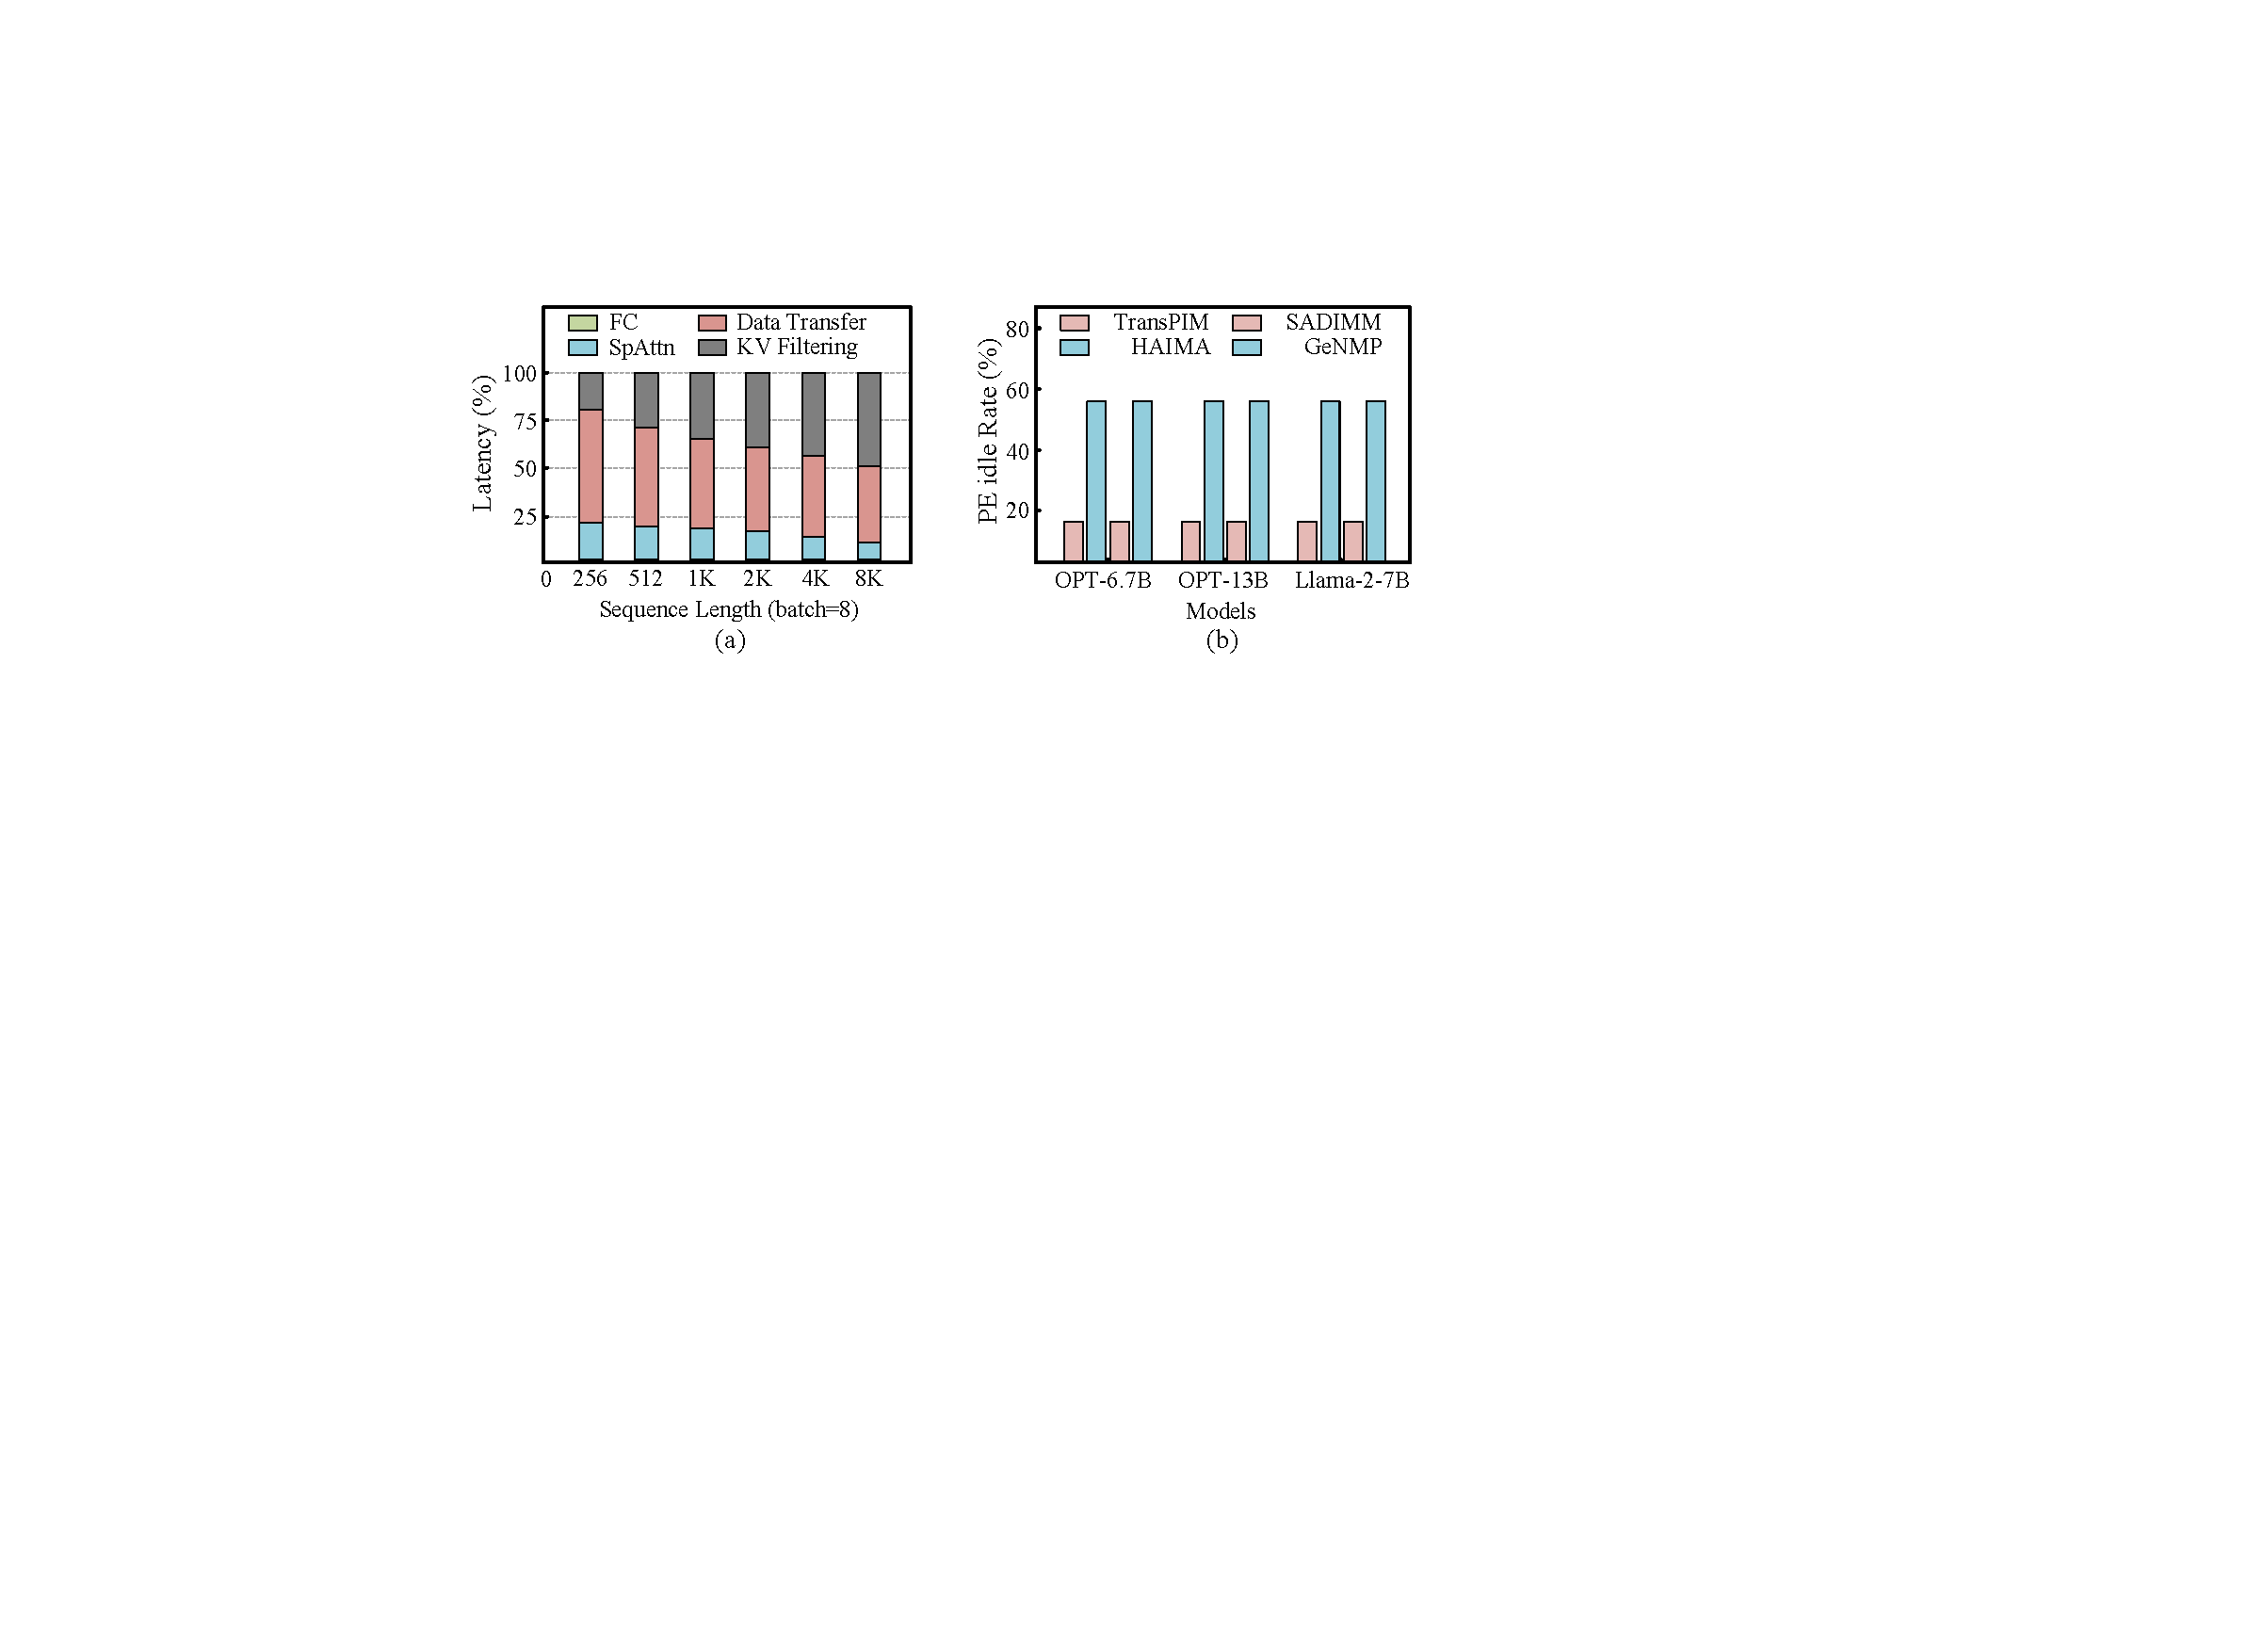
\includegraphics[width=8.3cm]{figures/exp/case2.pdf}
\vspace{-1em}
\caption{(a) PE idle rate comparison among SOTA NMP attention accelerators, (b) Data reuse rate comparison among SOTA NMP attention accelerators}
\label{case2}
\vspace{-2em}
\end{figure}

\textbf{Compared to Self-Attn.} In Figure~\ref{case1}(a), the bandwidth utilization of both MSDAttn and Self-Attn increases as the batch size grows. This suggests that a larger batch size enhances bandwidth efficiency and ensures fuller utilization of bandwidth. Figure~\ref{case1}(b) presents the cache hit rate of an NVIDIA A6000 GPU when processing MSDAttn and Self-Attn. Compared to Self-Attn, MSDAttn exhibits a significantly lower cache hit rate, which further declines as batch size increases. The strong data locality of Self-Attn arises from the principle that a token is more likely to have strong correlations with its neighboring tokens~\cite{longformer20}. Consequently, in global Self-Attn computation, neighboring token data can be extensively reused. In contrast, MSDAttn relies on highly irregular grid sampling, leading to poor data locality. Furthermore, different batches often involve distinct detection targets, rendering conventional locality-based data reuse strategies ineffective. As illustrated in Figure~\ref{case1}, MSDAttn substantially degrades deformable DETR’s performance, due to excessive memory bandwidth consumption driven by random memory accesses with poor data locality.


\subsection{Case Study\#2---MSDAttn With Modern NMPs}
\textbf{Configurations.} To identify the bottleneck of existing NMP accelerators for MSDAttn, we conduct a case study evaluating modern DETR models on \textit{state-of-the-art} (SOTA) NMP-based attention accelerators. Specifically, we examine three NMP-based accelerators: TransPIM~\cite{Zhou2022}, HAIMA~\cite{Ding2023}, and SADIMM~\cite{sadimm2025}. Since these accelerators are designed for Self-Attn, we introduce an additional module for these platforms to enable MSGS execution during simulation. Our study includes three DETR models, i.e., DE-DETR~\cite{zhu2021deformable}, DN-DETR~\cite{Li_2022_CVPR}, and DINO~\cite{zhang2023dino}. All models are running with object detection inference on the COCO 2017 dataset~\cite{Lin2014}. The data reuse rate is computed as follows: when a query's associated data is accessed for the first time, it is cached by the input buffer following a FIFO replacement policy. If a data block is not reused within the next four queries, it is evicted. The data reuse rate is given by $\frac{NMR-NRE}{NMR}$, where \textit{NMR} is the total number of memory requests, and \textit{NRE} is the number of input buffer replacements. The PE idle rate is calculated as follows: given $N$ processing elements (PEs) and a total execution time $T$ for the NMP accelerator. The execution time and stall time for PE$_i$ are denoted as $t_i$ and $s_i$ ($T = s_i + t_i$), respectively. The average stall ratio across all PEs is given by $\frac{\sum_{i=1}^{N}s_i}{NT}$.

\begin{figure}[t]
\centering
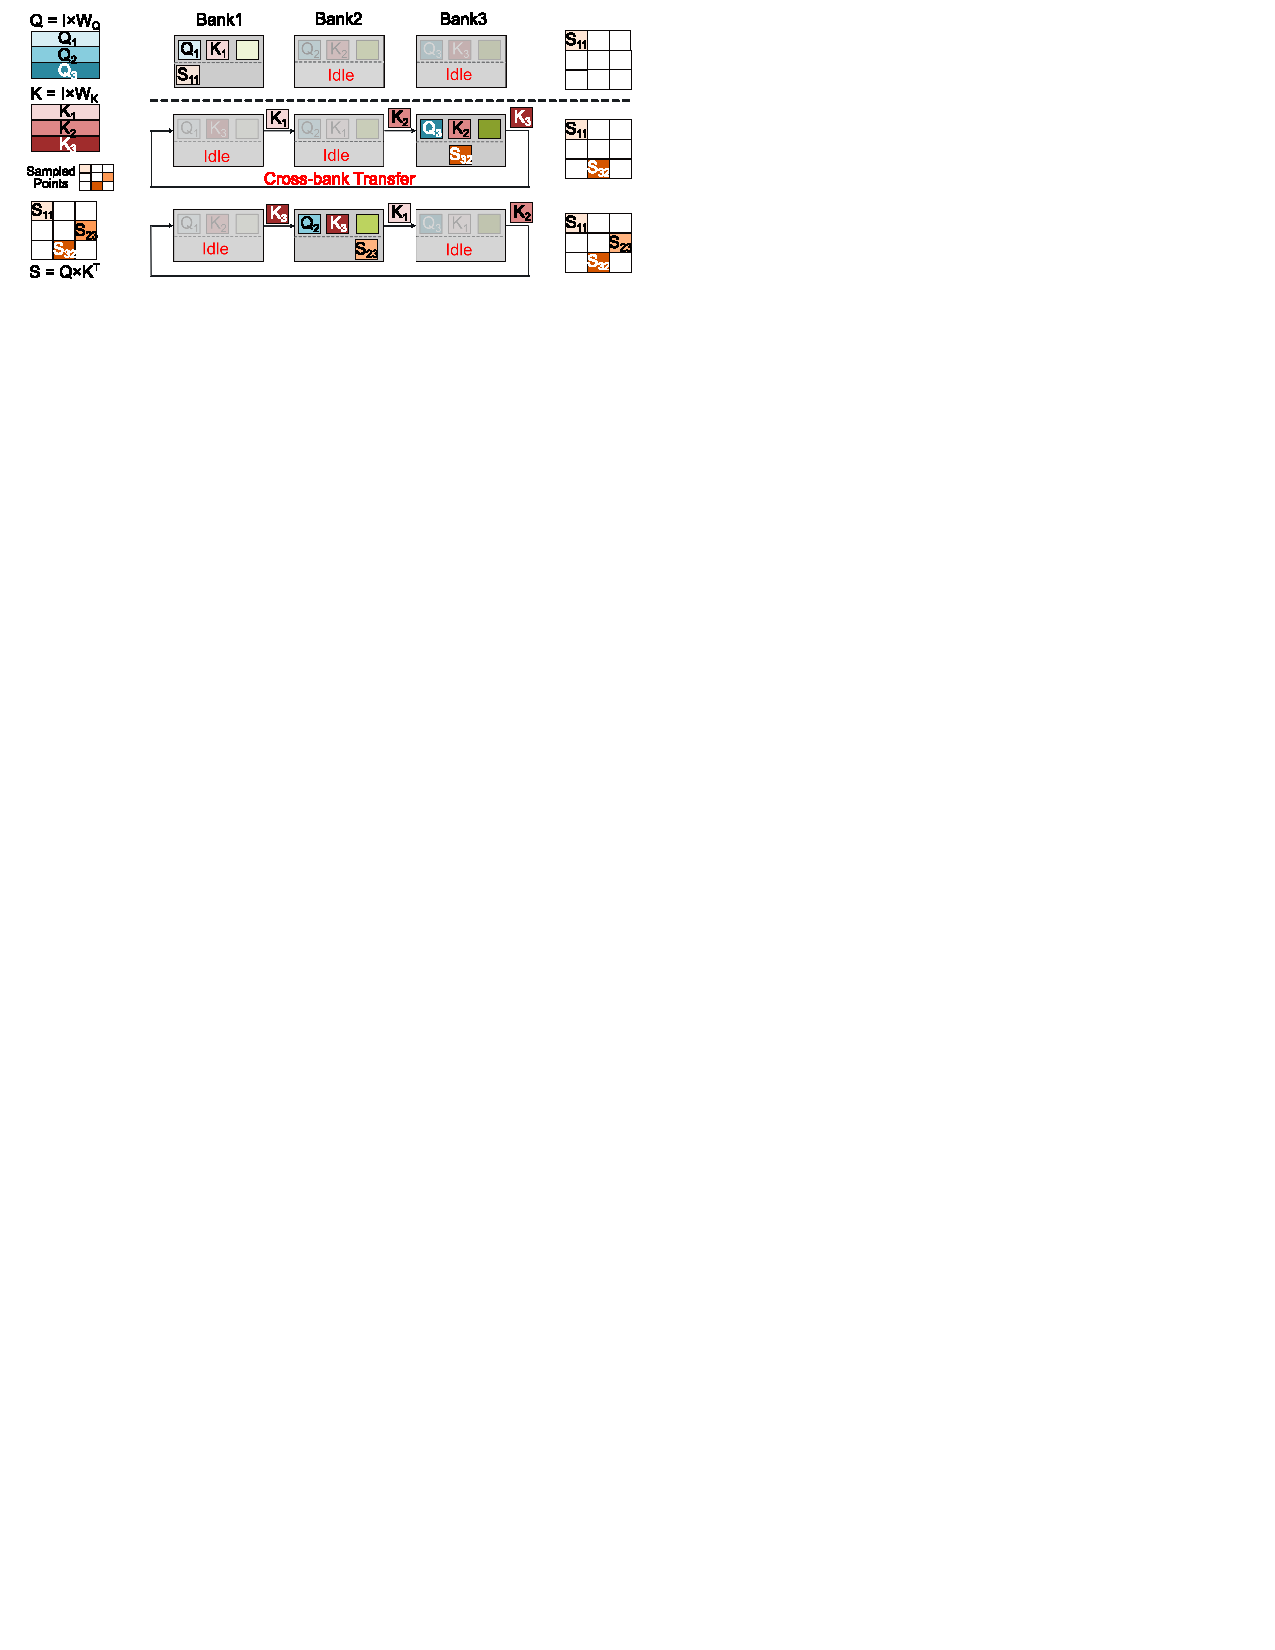
\includegraphics[width=8cm]{figures/graph/imbalance.pdf}
\vspace{-1em}
\caption{Many PE idle in TransPIM for sampled computing}
\label{imbalance}
\vspace{-1em}
\end{figure}


\textbf{Bottleneck\#1: load imbalance leads to PE idleness.} Figure~\ref{case2}(a) illustrates the PE idle rate for state-of-the-art NMP-based attention accelerators when executing DETR models, revealing that more than 50\% of PEs remain idle. This inefficiency is particularly evident in TransPIM~\cite{Zhou2022}, as shown in Figure~\ref{imbalance}, when applied to MSDAttn. TransPIM adopts a token-based dataflow, where tokens are partitioned and distributed across different memory banks. This approach is highly effective for self-attention, as it ensures high PE parallelism. However, when performing matrix computations with sampling, a significant number of PEs remain inactive. For instance, consider computing attention scores $S = Q \times K^\mathsf{T}$ using sampled elements $S_{11}$, $S_{23}$, and $S_{32}$ from matrix $S$. Although the storage of tokens across banks appears evenly distributed, the sampling operation bypasses most computations. As a result, in each iteration, only the PEs that contain the sampled data remain active, while others remain idle. This severe computational imbalance leads to substantial resource underutilization, limiting the efficiency of NMP-based accelerators when applied to MSDAttn.

\begin{figure*}[t]
\centering
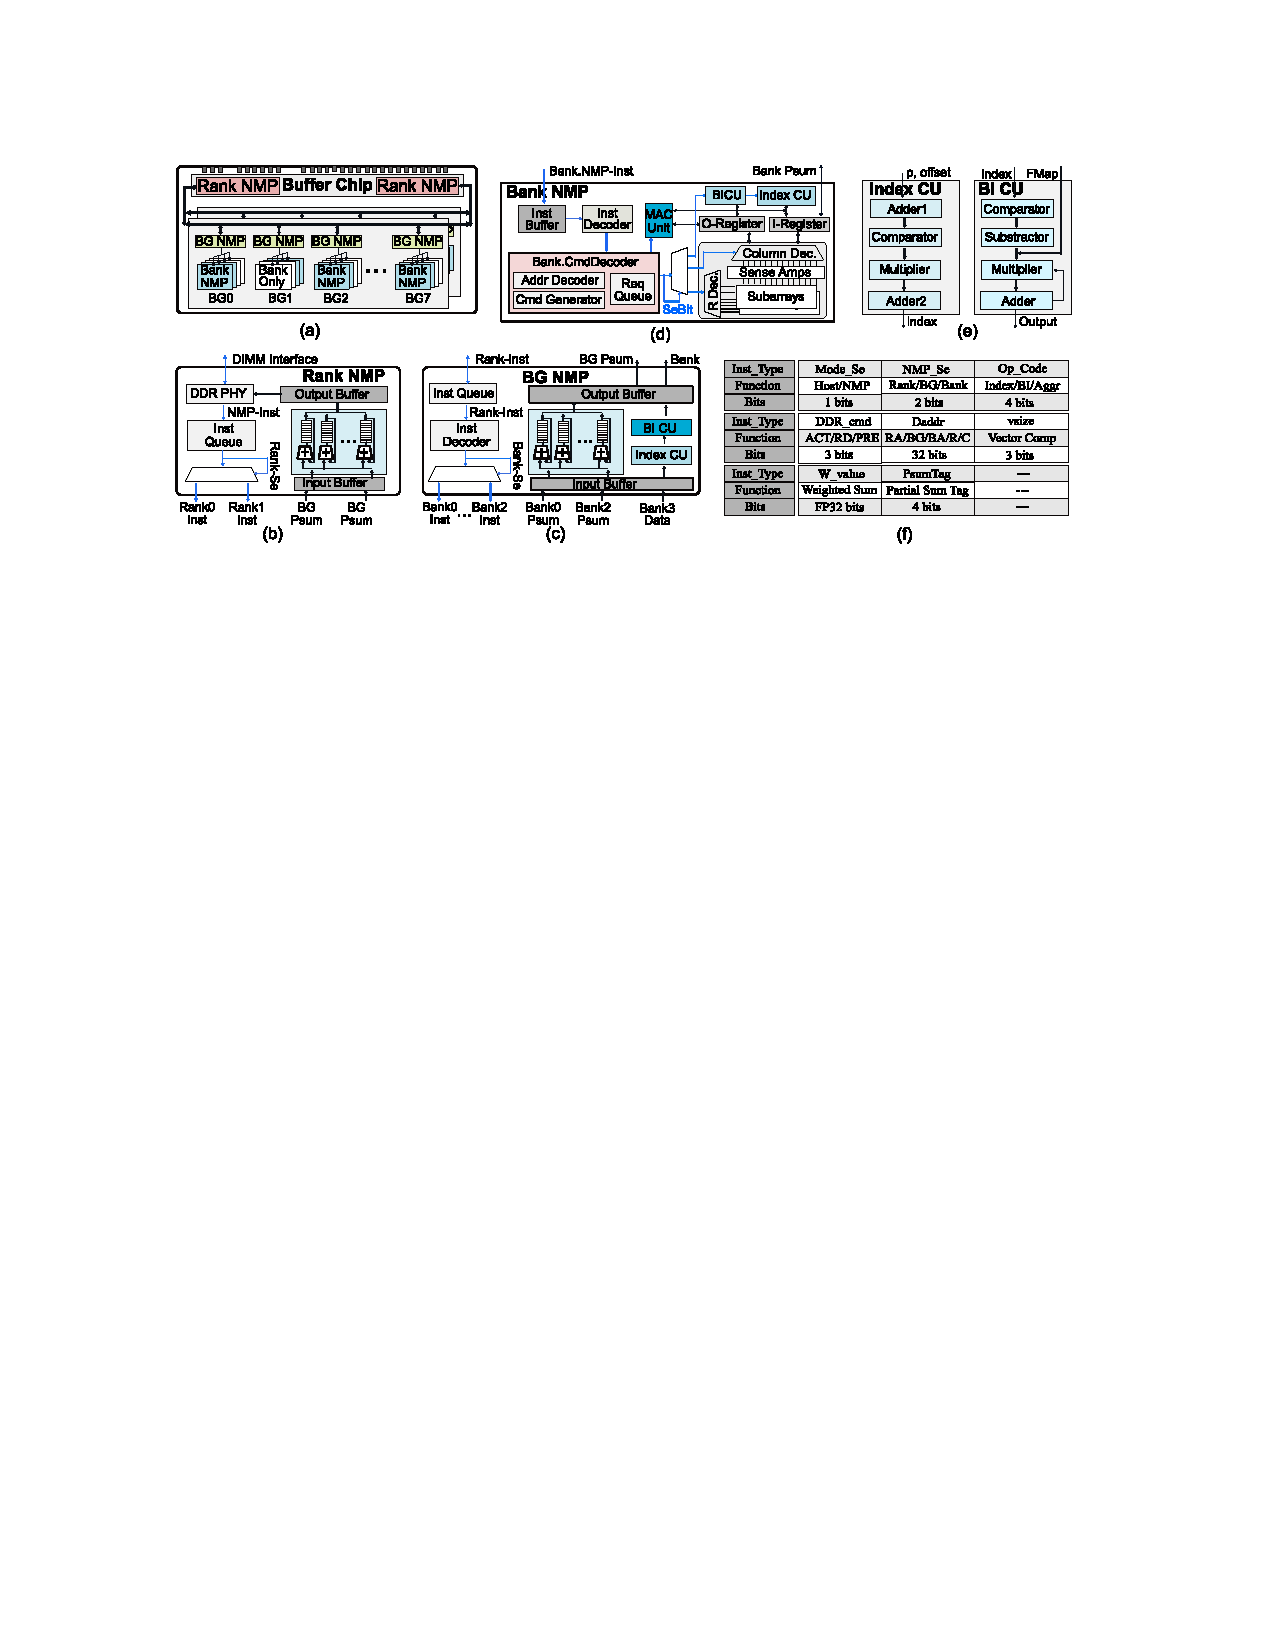
\includegraphics[width=16.5cm]{figures/graph/architecture.pdf}
\vspace{-1em}
\caption{(a) Architecture overview of \textit{DANMP}, (b) Rank-NMP, (c) Bank-group-NMP, (d) Bank-NMP, (e) Details of \textit{index computing unit} (ICU) and \textit{bilinear interpolation computing unit} (BICU), (f) NMP instruction format}
\label{architecture}
\vspace{-1em}
\end{figure*}

\textbf{Bottleneck\#2: poor data reuse leads to bandwidth waste.} Figure~\ref{case2}(b) depicts the data reuse rate of SOTA NMP-based attention accelerators on DETR models, showing a reuse rate of less than 20\%. To understand the root cause of this inefficiency, we analyze TransPIM’s design. TransPIM employs a token-based dataflow to improve data reuse. In the left part of Figure~\ref{imbalance}, the attention score matrix $S$ is computed as $S = Q \times K^\mathsf{T}$. Once $Q_1$ is multiplied by $K_1$, it can be immediately reused to compute $Q_1 \times K_2$, maximizing data locality. However, this reuse strategy fails when accelerating MSDAttn. The primary issue lies in MSGS, which exhibits poor data locality both within a single query and across multiple queries. \textit{Within a single query:} MSGS samples reference points from multiple orientations to capture diverse features, inherently limiting opportunities for data reuse. \textit{Across different queries:} Queries are processed in a random order, with varying detection targets, leading to minimal overlap between adjacent queries. As a direct consequence, a significant portion of memory bandwidth is wasted on repeatedly accessing irregularly sampled data, severely degrading system performance. Therefore, adapting NMP-based self-attention accelerators like TransPIM to MSDAttn is highly inefficient, as the lack of exploitable data locality negates the benefits of dataflow optimization techniques.

\begin{comment}

\begin{table*}
\centering
\tabcolsep=0.05cm
    \caption{Comparison among state-of-the-art NMP-based attention accelerators}
    \vspace{-1em}
    %\renewcommand\arraystretch{0.8}
    \label{tab:breakdown}
    %\tabcolsep=0.05cm
    \begin{tabular}{|c||c|c|c|c|}  
    \cline{1-5}
    
       {\bf Accelerators} & {\bf TransPIM~\cite{Zhou2022}}& {\bf HAIMA~\cite{Ding2023}} & {\bf SADIMM~\cite{sadimm2025}} & {\bf DANMP (this paper)}\\
       \hline\hline
       {\bf Hardware} & {HBM-based 2.5D integration}& {SRAM+DRAM near-memory} & {DIMM-based uniform PEs} & {DIMM-based irregular PEs}\\
       \hline
       {\bf Granularity} & {Token-based}& {Tile-based} & {DIMM-based} & {Sub-target-aware}\\
       \hline
       {\bf Load balancing} & {None}& {Static scheduling} & {\makecell{Dimension-based\\ data partitioning}} & {\makecell{Hardware-workload\\ co-matching}}\\
       \hline
       {\bf Sparse Support} & {Limited}& {Partial support} & {Support} & {Support}\\
       \hline
       {\bf Data reuse} & {Token reuse}& {SRAM reuse} & {Diagonal locality} & {\makecell{CAP improves spatial\\ and temporal locality}}\\
       \hline
       {\bf \makecell{Cross-bank\\ communication}} & {\makecell{Supported with\\ dedicated hardware}}& {\makecell{Relies on \\cross-bank access}} & {\makecell{Supported for\\ reductions}} & {\makecell{Avoided to reduce \\latency and energy}}\\
       \hline
       {\bf \makecell{Adaptability to\\ Complex Tasks}} & {Self-Attention}& {Self-Attention} & {Sparse attention} & {\makecell{\makecell{MSDAttn with\\ complex patterns}}}\\
       \hline
    
\end{tabular}
%\vspace{-1.5em}
\end{table*}[t]
\end{comment}



\subsection{Key Ideas of DANMP}
\label{key_idea}

%{While recent vision foundation models like LLaVA~\cite{liu2023visual} and Gemini~\cite{team2024gemini} rely on dense attention (e.g., ViT), deformable attention remains essential in tasks with geometric variability, long-range dependencies, or memory constraints---such as object detection~\cite{zhu2021deformable, Li_2022_CVPR, zhang2023dino} and 3D scene understanding~\cite{li2023dfa3d, mao2021voxel, kim2023voxel}. Our goal is not to replace dense vision transformers in general-purpose pipelines, but to improve the efficiency of sparse attention variants like MSDAttn, whose inductive biases and memory efficiency are advantageous in such domains. This focus is particularly relevant for edge AI, embedded vision, and spatially sparse tasks, where dense attention may be unnecessary or inefficient.}

Our first case study reveals that GPU-based MSDAttn suffers from severe memory bandwidth limitations, operating near the roofline. Consequently, leveraging NMP architectures to alleviate these bottlenecks is essential. Our second case study shows that existing NMP-based accelerators are ill-suited for MSDAttn. While current implementations typically offload both FC and self-attention layers, we find that the FC layer is compute-intensive with significant weight reuse. Thus, designing a dedicated NMP accelerator for MSDAttn is urgently needed.


%\textbf{Architecture Designs.} Our second case study observes that existing NMP architectures fail to meet the specific computational and memory access demands of MSDAttn. To address these limitations, we propose a new NMP architecture with three key design components. \textit{Lightweight Near-Memory Integration:} Since the compute-intensive FC layer does not require offloading, we adopt a lightweight integration strategy within memory, ensuring that MSDAttn’s computational needs are met while minimizing area and power consumption. \textit{Uneven Hardware Integration:} We design an unevenly integrated architecture for mapping irregular MSDAttn workloads to significantly reduce PE idleness without introducing cross-bank transfers. \textit{Custom Instruction Set:} We introduce a new instruction set tailored to support our novel architecture design, ensuring efficient execution of MSDAttn operations.

%\textbf{System Designs.} To efficiently support MSDAttn execution on NMP architectures, we introduce two key software-level optimizations. \textit{Clustering-and-Packing (CAP) for Data Reuse:} To increase data reuse, we propose a clustering-and-packing method that groups queries with similar sub-targets, thereby improving data locality and reducing random memory access overhead.
%\textit{Optimized Programming Model \& Execution Flow:} We design a new programming model and execution strategy specifically tailored for \textit{DANMP}, ensuring efficient scheduling and resource utilization in MSDAttn acceleration.



\section{DANMP Architecture Design}
\label{sec:architecture}

\subsection{Overall Architecture}

The overall architecture of \textit{DANMP} is illustrated in Figure~\ref{architecture}(a). It integrates three types of NMP units: near-rank PEs, near bank-group PEs, and near-bank PEs. The buffer chip contains two near-rank PEs responsible for managing I/O data transfers between two ranks. At the bank-group level, each group within a rank is paired with a dedicated PE, enabling near bank-group processing that enhances bandwidth utilization. Unlike prior NMP accelerators such as SADIMM~\cite{sadimm2025} and TransPIM~\cite{Zhou2022}, \textit{DANMP} selectively designates only a subset of banks (50\% based on the measured idle rate in Figure~\ref{case2}(a)) as bank-level NMP units instead of distributing computation across all banks. Each near-bank PE operates in local access mode, meaning it only accesses its corresponding bank (e.g., PE$_i$ exclusively accesses bank$_i$). Furthermore, \textit{DANMP} avoids cross-bank data transfers, a major source of bandwidth inefficiency. Such transfers not only require extra hardware, as in TransPIM~\cite{Zhou2022}, but also incur latency several times higher than local access.

As shown in Figure~\ref{msattention}, MSDAttn consists of two key operations: multi-scale grid sampling and aggregation of extracted features. These rely on three computational primitives—addition, multiplication, and reduction. Integrating \textit{DANMP} therefore requires including these primitives in hardware. A crucial design consideration is the optimal placement of logic units to handle MSDAttn’s varied demands efficiently. \textit{MSGS Execution:} Since MSGS frequently accesses feature maps and sampling points stored in memory banks, executing it with Bank-NMP minimizes latency and maximizes parallelism by keeping data local. \textit{Aggregation Execution:} Aggregation involves extensive reduction operations on interpolated and weighted results. As reduction naturally aligns with DIMM hierarchy, Rank-NMP and BG-NMP efficiently perform this task, leveraging DDR5 structure to optimize data flow and parallelism.


\subsection{Integration Details}
\label{integration_detail}


{\bf Rank-NMP Module.} The Rank-NMP module, shown in Figure~\ref{architecture}(b), integrates near-rank PEs to manage final data aggregation efficiently. In addition to performing standard DDR PHY functions, Rank-NMP serves as a transport layer for NMP control instructions, ensuring low-latency instruction propagation and execution synchronization. {The instruction queue size is limited to 5 because it shares the limited on-die area with NMP logic units. A larger queue can slightly improve packing efficiency but also increases area cost and reduces available compute resources. Through RTL validation, we found that a queue size of 5 achieves the best trade-off between packing benefit and hardware efficiency.} Instructions are multiplexed to specific ranks using the NMP-Select ($\mathtt{NMP\_Se}$) instruction. Rank-NMP aggregates results across all bank-groups. After each bank-group processes its local results (e.g., interpolated features or query partial sums), Rank-NMP performs final data aggregation and reduction. This process accumulates contributions from different feature map levels, forming the final attention-weighted feature vector. For multi-head attention, Rank-NMP also concatenates outputs from different attention heads. Since most arithmetic operations occur at the bank level, Rank-NMP only performs lightweight accumulation, ensuring minimal processing overhead. By finalizing aggregation at the rank level, \textit{DANMP} reduces the data volume sent to the host, improving bandwidth efficiency.


{\bf Bank-NMP Module.} The Bank-NMP module, illustrated in Figure~\ref{architecture}(d), handles MSGS near the bank's sense amplifiers, reducing latency and bandwidth usage. {It includes two primary components (Figure~\ref{architecture}(e)).} The \textit{Index Computation Unit (ICU)} calculates sampled coordinates from scaled reference points, performs boundary checks, and generates memory indices. Microarchitecturally, it comprises a coordinate sampler (Adder1), a comparator-based boundary checker, and an index generator (Multiplier and Adder2). The \textit{Bilinear Interpolation Computational Unit (BICU)} extracts fractional components, computes weights, and performs weighted summation over four neighboring pixels. It consists of a bitwise fraction extractor (Comparator and Subtractor), a multiplier, and a binary adder tree. Positioned near DDR5 sense amplifiers, Bank-NMP PEs perform low-latency memory accesses. Each PE directly computes interpolated features, eliminating raw pixel transfers over the bus. These PEs utilize SIMD-based MAC units for parallel processing. {As the MAC follows conventional architectures like Eyeriss~\cite{chen2016eyeriss}, we omit its internal structure for brevity.} Feature maps are partitioned so each bank holds a spatial tile, enabling bank-level parallelism (details in Section~\ref{sharding}).

{\bf BG-NMP Module.} The BG-NMP module (Figure~\ref{architecture}(c)) acts as a bridge between Rank-NMP and Bank-NMP, aggregating intermediate results while managing bilinear interpolation for non-PE banks. Given the hierarchical nature of DRAM, batch-wise reduction operations are efficiently executed at the bank-group level before forwarding the aggregated data to Rank-NMP for final processing. BG-NMP also coordinates indexing computations, ensuring that near-bank PEs handle hot data within the nearest bank, while bank-group PEs process cold data from all its non-PE banks. Compared to even integration, this approach reduces costly hot data transmission from with-PE bank to non-PE bank, preventing unnecessary movement (cross-bank transfer) of raw pixel data. {To support these functions, each bank-group integrates accumulator, ICU, and BICU units, where the ICU and BICU contain dedicated adder and multiplier arrays capable of performing vector-level MAC operations.} Additionally, BG-NMP balances workloads by distributing simple, localized computations to individual banks while managing cross-bank coordination at the bank-group level. This structure maximizes parallel processing while keeping computations close to the data, ensuring optimal memory efficiency and performance.


%{\bf Figure Clarifications.} To improve clarity, we have explicitly described the components shown in Figure~\ref{architecture}(b)–(d). The {\em Inst Buffer} in Figure~\ref{architecture}(d) receives decoded instructions from the bank-group instruction decoder, which specify whether each operation (e.g., interpolation, accumulation, or reduction) should be executed by local PEs or by the BG-level unit. The {\em SeBit} denotes the row-selection signal within the DRAM array, controlling which wordline is activated for each memory access. The adders shown in Figures~\ref{architecture}(b) and (c) serve as reduction units that accumulate intermediate results collected from multiple banks before forwarding them to higher-level aggregators.


%{{\bf Comparison with Workload-aware NMPs.} Prior NMP accelerators like HAIMA~\cite{Ding2023} and SADIMM~\cite{sadimm2025} employ workload-aware integration by embedding different logic units across the memory hierarchy. HAIMA separates compute units between SRAM and DRAM to handle distinct tasks, while SADIMM performs coarse-grained specialization at the near-bankgroup and near-bank levels. However, both use uniform logic units across all banks, ignoring spatial workload variation. In contrast, \textit{DANMP} adopts a fine-grained, bank-level non-uniform PE integration strategy, placing processing elements in only a subset of banks. To our knowledge, \textit{DANMP} is the first NMP accelerator to support such non-uniform bank-level integration, which is critical for efficiently handling MSDAttn’s highly irregular memory access patterns.}

{{\bf Technical Feasibility of Non-Uniform PEs.} While traditional DRAM (e.g., DDR4/5) employs symmetric bank configurations for manufacturing and interface compatibility, recent research demonstrates the feasibility of heterogeneous designs across banks and subarrays. FIGARO~\cite{wang2020figaro} enables subarray-level partitioning into fast and slow regions using a shared global row buffer. CROW~\cite{hassan2019crow} introduces "regular" and "copy" rows within subarrays, activated independently via additional decoder logic to accelerate hot rows. LISA~\cite{chang2016low} adds lightweight inter-subarray links and identifies fast segments for in-DRAM caching, enabling intra-bank latency heterogeneity. These efforts show that DRAM can be configured at fine granularity, such as banks and subarrays, supporting the non-uniform PE integration strategy proposed in this work.}



\subsection{NMP Instruction Format}
\label{instruct}
{\bf Overview.} {Similar to RecNMP~\cite{recnmp2020} and ReCROSS~\cite{Liu2023},} the \textit{DANMP} accelerator uses a 83-bit compressed instruction format that tightly encodes memory and compute operations. This format was designed to fit within standard memory interface constraints. We refine and elaborate each field of the instruction to better support advanced operations, e.g., indexing, bilinear interpolation, aggregation, weighted sums.

{\bf Instruction Format Breakdown.} The fields and their typical bit widths are shown in Figure~\ref{architecture}(f). \textit{Mode Selection:} The 1-bit $\mathtt{Mode\_Se}$ indicates the memory working on DRAM mode or NMP mode. {In \textbf{DRAM mode}, data remain striped across chips and accessed via host controller. In \textbf{NMP mode}, each bank issues local requests through its embedded PE and executes independently. Feature tiles are remapped into per-bank scratchpads under a separate logical address space, invisible to the host, preserving full DRAM compatibility.} {\textit{NMP Selection:} The 2-bit $\mathtt{NMP\_Se}$ determines whether an instruction is executed by the near-rank PEs, near bank-group PEs, or near-bank PEs. This classification is generated by the host-side memory controller based on operation types.} \textit{Operation Type:} The 4-bit $\mathtt{Op\_Code}$ covers sum/mean ($\mathtt{NMP\_Sum/Mean}$), weighted sum ($\mathtt{NMP\_WSum}$), bilinear interpolation ($\mathtt{NMP\_Interp}$), etc. \textit{DDR Command Flags:} The 3-bit $\mathtt{DDR\_cmd}$ compresses the DRAM commands (Activate, Read, Precharge) needed for the memory access. The memory controller (host) or the near-rank controller sets these flags based on whether the target row is already open, how many column bursts are needed, etc. 
%This compression lets one NMP instruction trigger a sequence of DRAM operations internally, instead of sending each command over the bus.

\textit{Memory Address:} The 32-bit $\mathtt{Daddr}$ supplies the memory location for the operation. In a DRAM setting it can be broken into rank, bank-group, bank, row, and column bits. \textit{Vector Size/Length:} The 3-bit $\mathtt{vsize}$ influences how many DRAM column bursts the rank controller issues. \textit{Weight Field:} The 32-bit $\mathtt{W\_value}$ supplies the scalar weight to multiply the fetched vector by for weighted sum opcodes. \textit{Partial Sum Tag:} The 4-bit $\mathtt{PsumTag}$ identify which accumulation stream this instruction belongs to. This is crucial for aggregation/reduction operations. Only data with the same $\mathtt{PsumTag}$ will be accumulated, ensuring the correctness of the reduction operation.

%If the operation is unweighted, this field can be repurposed. For example, in a bilinear interpolation mode, the 32-bit field could be split into two 16-bit fractional weights (for the X and Y interpolation ratios) instead of a single multiplier.

% This entire flow is controlled by synchronized instructions – for example, a single high-level “compute attention” command might trigger a predefined sequence in the near-rank controller, which in turn coordinates lower-level operations with minimal handshaking. The instruction propagation is hierarchical broadcast: one command from the rank fan-outs into multiple bankgroup commands, which further fan-out to multiple bank operations. Because each level has its own simple controller, the scheduling can be optimized locally (each bankgroup knows to wait for all its banks to finish, etc., without burdening the global controller with those details). This hierarchical control reduces overhead and scales well: adding more banks or groups doesn’t linearly increase complexity at the top.



\section{DANMP System Design}
\label{system}

\subsection{Data Sharding and Mapping}
\label{sharding}
To leverage DDR5’s high bank-level parallelism, feature maps and attention weights are evenly distributed across DDR5’s 32 banks, organized into 8 bank-groups. This partitioning ensures maximum concurrent access by minimizing contention. For instance, a query's sampling points are placed in separate banks to prevent overloading and enable parallel fetching. The four neighboring pixels of a sampling point are stored in the same bank to reduce cross-bank overhead. However, while this tile-based mapping prevents bank conflicts, it introduces load imbalance. Despite equal storage, pixel access probability varies significantly; for example, in portraits, the facial region sees higher sampling, causing uneven workloads.

To address this, we implement a coordinate clustering approach before mapping feature maps to banks. Specifically, query-related coordinates are first computed and clustered to identify frequently sampled regions. {DANMP classifies feature entries by access frequency: the top 50\% most frequently accessed entries are mapped to PE-equipped banks for local computation, while the remaining 50\% are evenly assigned to the banks without PEs.} This frequency-based mapping ensures balanced utilization without overloading PE banks. Since these infrequently accessed data are typically stored across different banks, we use near bank-group PEs to process them, thereby reducing cross-bank data transfers. This optimized mapping strategy incurs minimal overhead, as the coordinate clustering approach operates solely on coordinate data and does not require feature map access or interpolation operations. 
%By balancing computational workload across banks while maintaining high memory access parallelism, \textit{DANMP} achieves efficient and scalable near-memory processing for MSDAttn acceleration.


\subsection{Clustering-and-Packing Algorithm}
\label{capa}
\textbf{Current Challenges in Data Reuse.} In a single DETR query, pixels from various orientations are sampled to capture richer features. However, this process inherently results in low data reuse due to the lack of spatial locality. When executing a batch of queries on a single feature map, data reuse opportunities remain limited for two primary reasons. First, different queries typically correspond to distinct detection targets, which are randomly distributed across the feature map. Second, the arrival order of queries is entirely random, leading to poor temporal locality and further hindering efficient data reuse. Addressing these challenges is critical to minimizing redundant memory accesses and improving system performance.


\textbf{Opportunity Analysis.} Although queries generally focus on different detection targets, many targets can be decomposed into smaller sub-targets, often leading to overlaps across queries. For instance, in portrait detection, detecting both the upper body and face involves extracting common facial features. If queries with shared sub-targets can be identified, spatial locality can be leveraged to enhance data reuse. However, random query order greatly undermines this benefit. For example, after detecting a face, if subsequent queries focus on unrelated objects, the cached facial features may be evicted from the buffer. Consequently, when the system later detects the upper body, it cannot reuse previously computed facial features. To maximize data reuse, queries with shared sub-targets should be grouped to improve temporal locality. This strategic grouping keeps frequently accessed data available for reuse, reducing memory access and improving performance.

\begin{algorithm}
\caption{Clustering-and-Packing}\label{alg:sap}
\begin{algorithmic}[1]
\Require \textit{Q}, \textit{V}, $W^{S}$ are query, FMap and weight matrices, 
$P(x,y)$ is the coordinate set of all reference points
\Ensure Bilinear Interpolation (\textbf{BI}) of sample points $p+\Delta p$
\State $\hat{Q}$ $\leftarrow$ Random selecting 20\% queries from $Q$
\State $\Delta\hat{p}$ = $\hat{Q}\times W^S$
%\State Output $\leftarrow$ \textbf{BI}(V, $\hat{p}+\Delta \hat{p}$)
\State $k\times$ Cluster Centroids $C$ $\leftarrow$ \textbf{K-means}($\hat{p}+\Delta \hat{p}$)
{\State Mapping feature values of $9\times 9$ pixels near $C$ to banks with PE}
\While{$q \in (Q-\hat{Q})$ ($i=0$)} 
\State $\Delta p = q\times W^S$
\State $j^{th}$ Cluster Centroid $C_j$ $\leftarrow$ \textbf{Search}($C$, $p+ \Delta p$)
\State Pack$_j$ = \textbf{Packing}($p+ \Delta p$), $i++$
\EndWhile
\State Output $\leftarrow$ \textbf{BI}(V, from Pack$_0$ to Pack$_k$)
\end{algorithmic}
\end{algorithm}


\textbf{Algorithm Details.} Algorithm~\ref{alg:sap} outlines the CAP method for improving data reuse in bilinear interpolation. {\textit{Random Query Selection (Lines 1-2):} 20\% of queries from the same FMap are randomly selected to compute sampled point offsets $\Delta\hat{p}$. \textit{Clustering (Line 3):} K-means clustering is applied to the sampled points ($\hat{p} + \Delta\hat{p}$), yielding $k$ cluster centroids. A $9\times9$ pixel region is used as the clustering distance metric, identifying frequently accessed (hot) regions. Since only coordinates are involved, this step can be performed prior to FMap storage. The feature values around each cluster center are stored in PE-equipped banks (hot entries), while the rest are placed in non-PE banks (cold entries). \textit{Query Packing (Lines 4-8):} For the remaining 80\% of queries, offsets are computed as $\Delta p = q \times W^S$. Each sampled point ($p + \Delta p$) is mapped to its nearest cluster centroid. Queries targeting the same $9\times9$ region are grouped into packs, enabling shared sub-targets and improved data reuse. \textit{Optimized Bilinear Interpolation (Line 9):} Query packs undergo bilinear interpolation collectively, maximizing reuse and improving efficiency.}


%{\bf Hierarchical Load Balancing.} To explicitly address the load imbalance issue discussed in Figure~\ref{imbalance}, \textit{DANMP} adopts a two-level strategy operating across and within bank-groups without cross-bank migration. At the {\em inter-bank level}, coordinate clustering maps frequently accessed (hot) regions (balanced loads) to PE-equipped banks for local execution, while less active (cold) regions are placed in non-PE banks. At the {\em intra-bank-group level}, BG-NMP directly executes interpolation, weighted accumulation, and partial reduction on behalf of its non-PE banks, effectively acting as their computation proxy. As a result, all computations are consolidated to PE-equipped banks and BG units, achieving balanced utilization and avoiding costly cross-bank data transfers. This design, combined with CAP-based query packing, smooths temporal burstiness and transforms MSDAttn’s skewed access pattern into a balanced, high-throughput execution flow.


%{{\bf Online Deployment Considerations.} While CAP improves data reuse across queries within a single FMap, it is not intended for reuse across frames in a video stream. Although object queries may target similar semantics across adjacent frames, their sampling coordinates often shift due to object or camera motion. Since CAP clusters queries based solely on spatial proximity, such variation limits cross-frame reuse. Therefore, we recommend applying CAP on a per-frame basis, with clustering performed independently for each frame. CAP initialization involves only lightweight coordinate computations (not feature values) and is efficient at runtime. As shown in Figure~\ref{latency_break}(a), CAP contributes less than 2\% of total inference time, making its overhead negligible for online deployment. While CAP organizes queries for reuse-aware execution, it avoids global synchronization. Queries outside clustered regions (i.e., the 9$\times$9 window) proceed immediately, while those in packs are processed incrementally. To avoid excessive delay, we impose a maximum wait time (e.g., 64 cycles) per pack, after which all pending queries are processed. This hybrid scheduling boosts data reuse without introducing significant latency for time-sensitive queries.}

%\textbf{Trade-off Analysis.} Compared to the traditional MSGS algorithm, our approach introduces two additional overheads. \textit{K-means Clustering Overhead:} We introduce a K-means clustering phase to detect potential data reuse opportunities. {\textit{Nearest Cluster Center Search Overhead:} Each query requires finding its nearest cluster center. To accelerate this, we build a reverse-encoded lookup table during CAP initialization. For each cluster center $C_j$, its $9\times 9$ coverage region is rasterized into a 2D array (cluster\_map) indexed by spatial coordinates. All pixels in cluster\_map share the same cluster ID, enabling constant-time ($O(1)$) region checks by first retrieving the cluster ID and then verifying inclusion in the $9\times 9$ area. This eliminates the need for runtime comparisons across the entire FMap. The memory overhead of this table is under 256KB for a $4096\times 4096$ FMap.} Despite these overheads, the advantages of our proposed algorithm are substantial. By grouping queries that share sub-targets, our method significantly improves data reuse between adjacent queries. This reduces the high-volume random memory accesses that are inherent in MSGS. {Figure~\ref{softonly}, Figure~\ref{latency_break}, Section~\ref{hard_soft}, and Section~\ref{lea_break} also provide experimental evidence that the introduction of the CAP algorithm brings more benefits than drawbacks.}

%Similar to previous NMP architectures~\cite{recnmp2020, chen2023}, \textit{DANMP} follows a heterogeneous computing programming model. In this model, application execution is divided between host-side operations running on the CPU and NMP kernels executed on \textit{DANMP} PEs. The NMP kernels are compiled into packets of NMP instructions (NMP-Insts) and transmitted to each memory channel via the DIMM interface, directing them to the corresponding \textit{DANMP} PEs. 

\subsection{Programming Model and Execution Flow}
\label{execution_flow}
{\bf Overview.} At the core of DANMP's programming model, the CPU serves as the system’s central controller, managing global information and orchestrating execution, while NMP units focus solely on executing assigned computations and returning results. Several global factors are critical to ensuring efficiency, including: (1) the distribution of near-bank PEs, (2) the spatial distribution of sampling points, and (3) cluster center information from the CAP algorithm. To illustrate, consider a feature map: the CPU first calculates sampling point locations for 20\% of queries and applies CAP clustering to identify frequently accessed (hotspot) regions. Using this information, the CPU issues instructions to store hotspot-associated feature map segments in banks with PEs, while non-hotspot regions are allocated to banks without PEs. For the remaining 80\% of queries, once the CPU determines sampling point coordinates, it performs query packing to enhance temporal locality, improving data reuse. Finally, based on the spatial distribution of sampling points, the CPU generates instructions for different NMP levels to optimize execution.

\begin{figure}[t]
\centering
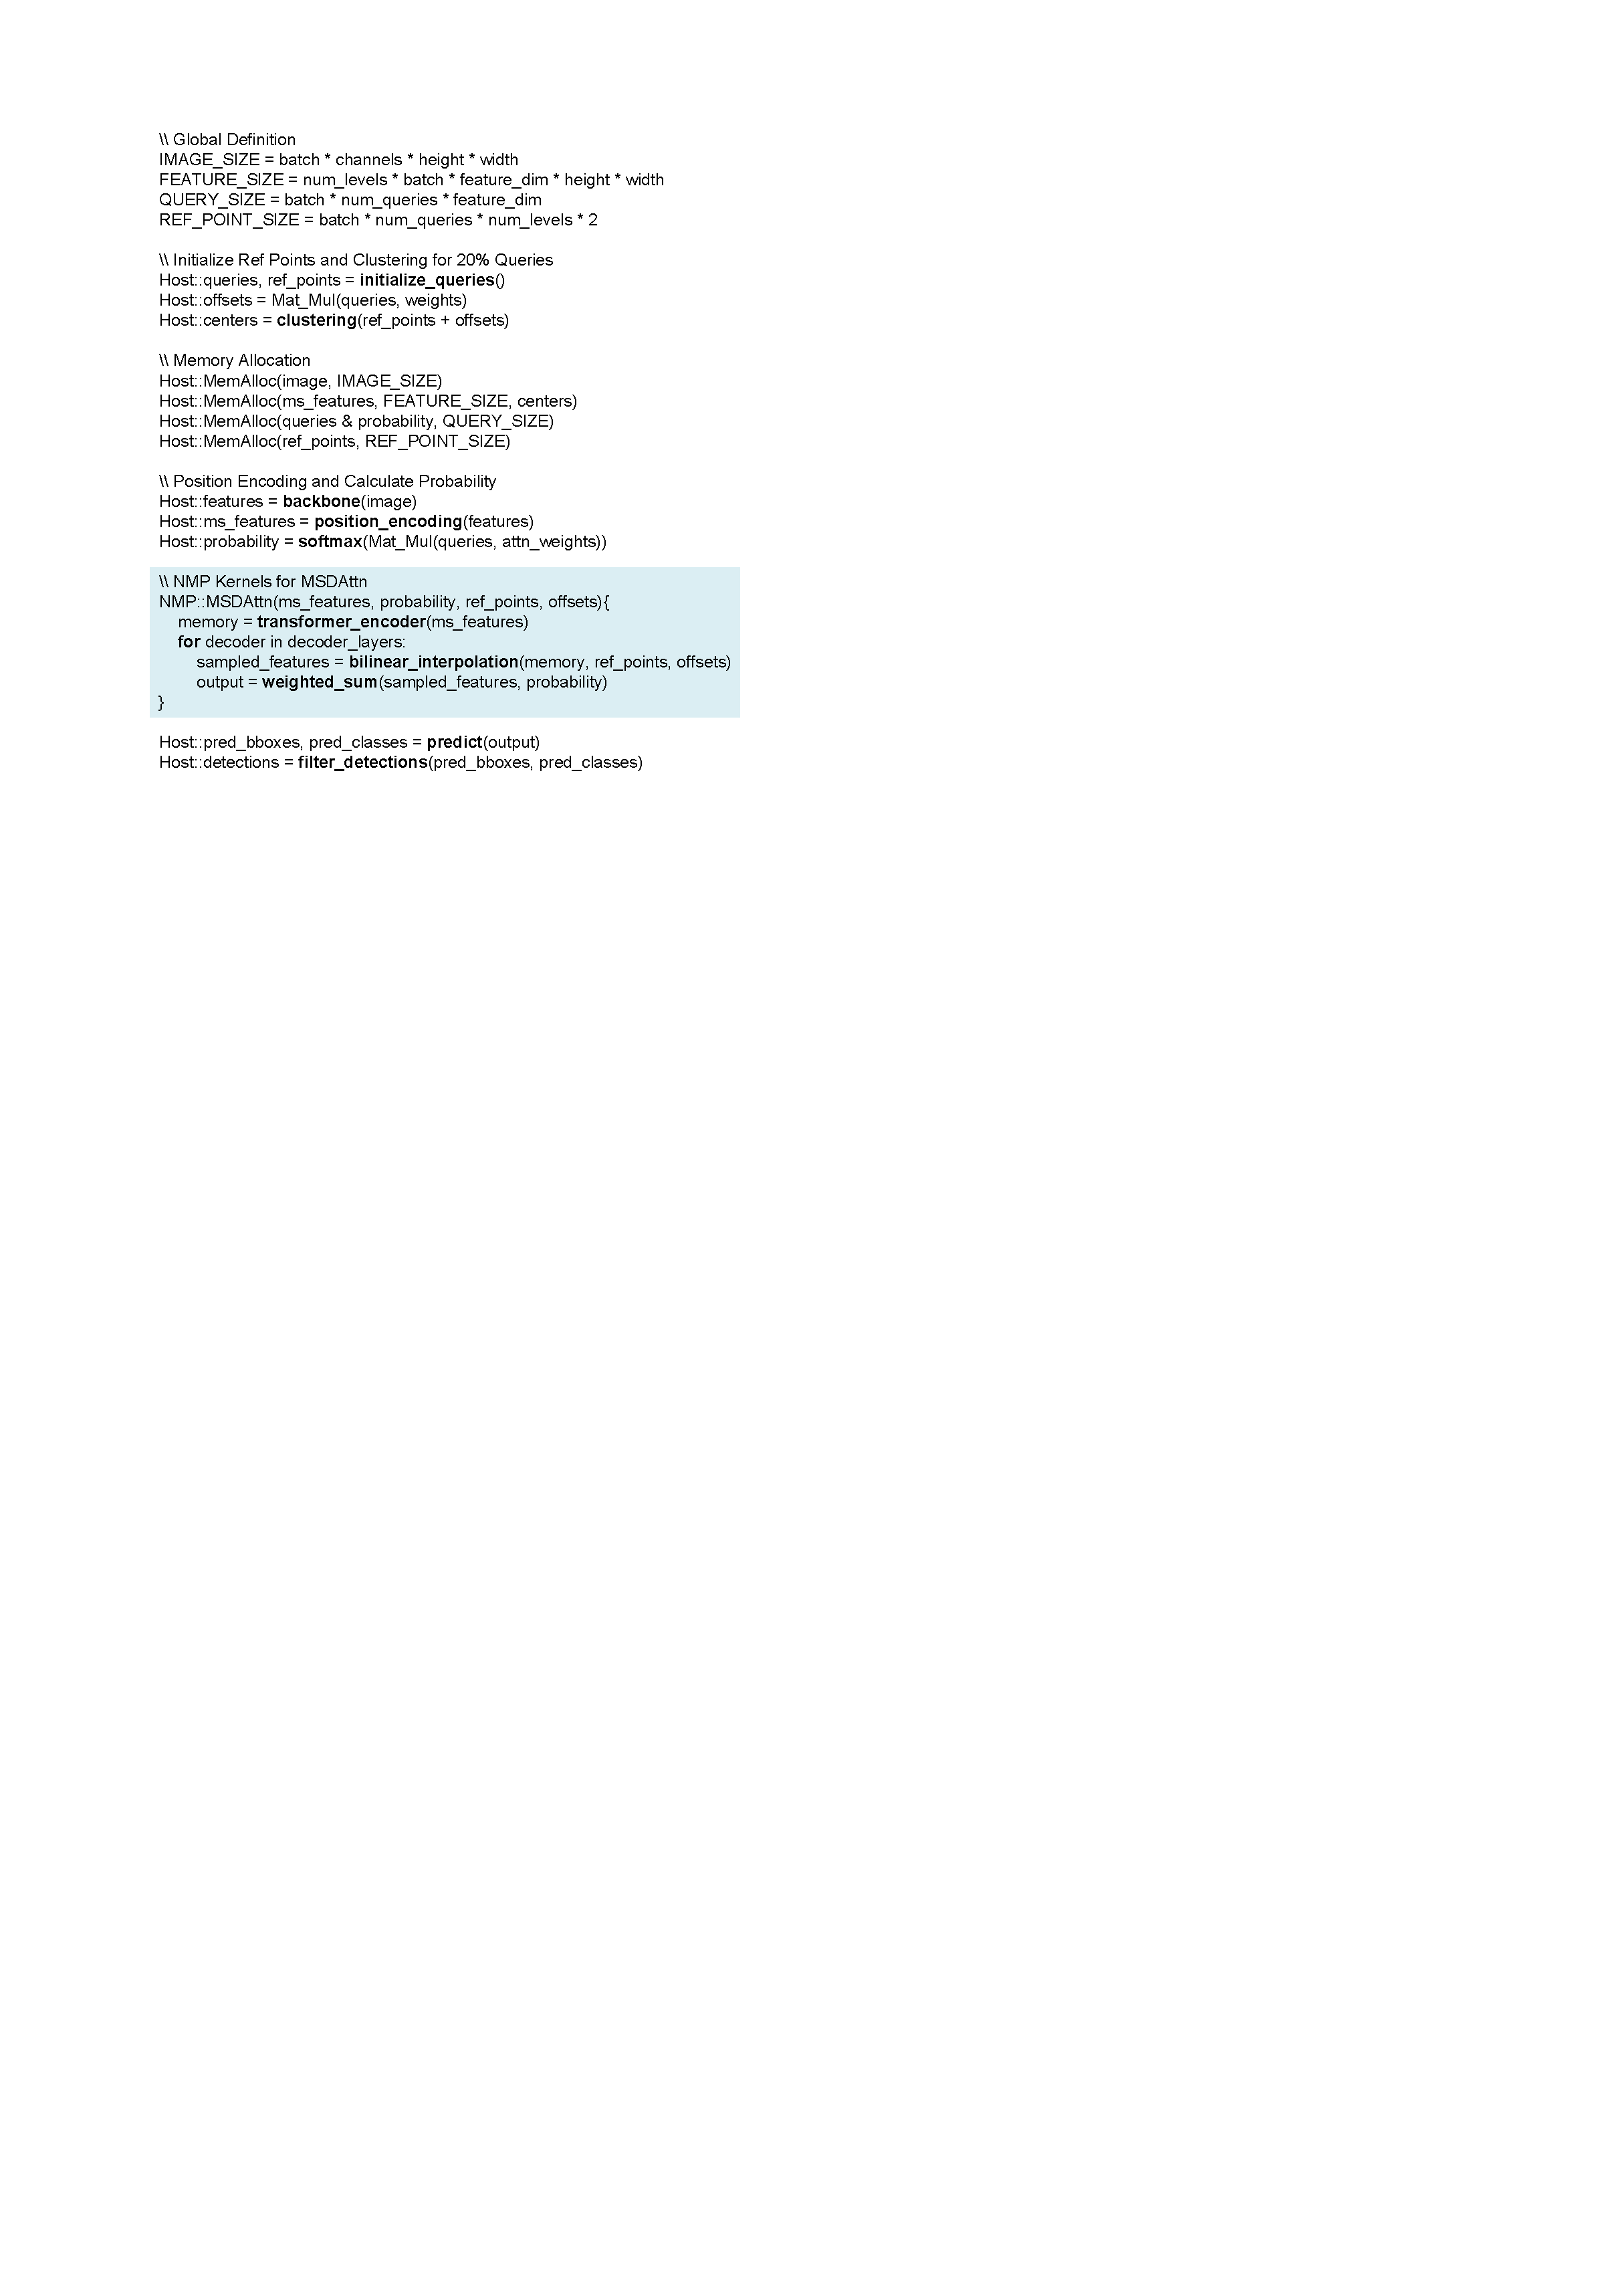
\includegraphics[width=8.1cm]{figures/graph/code.pdf}
\vspace{-1em}
\caption{\textit{DANMP} MSDAttn example code}
\label{code}
\vspace{-1.5em}
\end{figure}

{\bf Details of DANMP's Execution Flow.} Figure~\ref{code} presents an example code of host-\textit{DANMP} collaborative processing for DETR inference. The blue region highlights the MSDAttn portion that needs to be offloaded to \textit{DANMP} for execution. We use Figure~\ref{architecture} to elaborate on the detailed process of executing MSDAttn with \textit{DANMP}. The control logic is designed to keep all levels of the hierarchy busy. While one set of sample points is being processed at the banks, the near-rank unit can prepare the next set of instructions, overlapping computation and communication. The execution sequence for one detection query is as follows.

(1) The near-rank NMP receives the NMP instructions of one query, which contains all the informations shown in Figure~\ref{architecture}(f). (2) The near-rank instruction decoder will broadcast the instruction info down to the bank-groups according to the $\mathtt{NMP\_Se}$ field. (3) If $\mathtt{NMP\_Se} = bank$ and the instruction is successfully broadcast to all banks, the banks equipped with PEs will proceed with memory access based on the address specified by $\mathtt{Daddr}$. If $\mathtt{NMP\_Se} = bank-group$, The near-bank-group instruction decoder will collect data from its banks with $\mathtt{Daddr}$. Then the PEs within the bank-groups will generate the bilinear interpolation results locally. (4) Near-bank PEs will collect data from the input buffer in Figure~\ref{architecture}(d). Meanwhile, the near-bank instruction decoder will parse the $\mathtt{Op\_Code}$ field to determine the specific operation to be executed. (5) After the local execution of parallel near-bank PEs, those partial results are sent over a fast intra-bank-group bus to the near-bank-group PE, which adds them together. (6) Each bank-group PE then sends its result (e.g., one interpolated feature vector per sample or a partial sum for the query) up to the near-rank unit. (7) The near-rank unit accumulates all these vectors into the final output for the query's attention computation, and writes it to a designated location or return it to the host.


%{\bf Efficient Scheduling.} The accelerator's control logic is responsible for dynamic scheduling, ensuring efficient load balancing. If certain bank-groups complete their tasks early, such as when a particular feature scale has fewer sampling points or is easier to fetch, the near-rank unit can immediately assign them new tasks, rather than waiting for all bank-groups to reach a synchronization barrier. To maintain correctness in reduction operations, \textit{DANMP} employs $\mathtt{PsumTag}$, a tagging mechanism that assigns the same identifier to partial sums requiring aggregation. The near-rank PE accumulates only those partial sums with matching $\mathtt{PsumTag}$ values. {To support dynamic scheduling, each rank includes a centralized scheduler and lightweight per-bankgroup task queues. When a bank-group finishes processing a task, it signals the scheduler, which immediately assigns a new task from the queue, avoiding global synchronization barriers.} Additionally, \textit{DANMP} leverages the structured computation pattern of MSDAttn to enable parallel execution across scales and attention heads. Multi-scale deformable attention naturally supports inter-level parallelism, where different feature scales can process sampling points concurrently on separate bank-groups. The controller schedules these operations in parallel to prevent bank idleness, as each feature scale is mapped to distinct banks. 

%Furthermore, \textit{DANMP} ensures precise execution ordering for critical computations: (1) Address parsing and memory fetches occur at the bank level. (2) Multiplications and local summations take place at the bank or bank-group level. (3) Final accumulation of attention scores is performed at the rank level. By carefully orchestrating these steps, the architecture effectively eliminates pipeline stalls and optimizes memory utilization. Control instructions propagate downward, carrying essential execution parameters (e.g., memory addresses, offsets, and operators), while status updates and computed results flow upward. This streamlined execution model minimizes control overhead, as most scheduling and address parsing occur only once, while actual data movement and arithmetic operations are fully handled by hardware, eliminating the need for frequent CPU intervention.



\section{Evaluation}
\subsection{Experimental Setup}
\label{exp_setup}
{\bf Simulation Framework.} Table~\ref{tab:config} summarizes the core simulation settings used for evaluating the performance of \textit{DANMP}. We conduct a cycle-accurate, full-system simulation of a 32-core architecture with a DDR5-based memory hierarchy. Processor cores and the cache subsystem are modeled using the gem5 simulator~\cite{gem5}, which captures instruction-level behavior, cache interactions, and memory access patterns. To model the memory subsystem, including DDR5 channels and near-memory logic, we extend Ramulator~\cite{ramulator2015} with a custom NMP simulation backend. This extension incorporates cycle-level models for address translation, NMP-specific instruction generation, and detailed execution timing of \textit{DANMP}'s processing elements (PEs). Hardware synthesis of the PEs targets a 40nm CMOS process at 300MHz, matching the internal frequency of DDR5-4800. For area and power estimation of the NMP logic, we utilize Synopsys Design Compiler. Memory access energy and I/O power are derived using CACTI-3DD~\cite{CACTI-3DD} and CACTI-IO~\cite{CACTI-IO}, respectively. 
%All collected energy parameters are integrated into the simulation to provide fine-grained power and energy tracking.

\begin{table}[t]
\centering
\tabcolsep=0.12cm
    \caption{System Parameters and Configurations}
    \vspace{-0.5em}
    %\renewcommand\arraystretch{0.8}
    \label{tab:config}
    %\tabcolsep=0.05cm
    \begin{tabular}{c|c|c|c}  
    \hline\hline
       \multicolumn{4}{c}{\bf Host-side CPU Configurations} \\ \hline
       {Processor} & {32 Cores, 2.5GHz} & {L1 Caches} & {32KB per core}  \\
       \hline
       {L2 Caches} & {1MB per core} & {Shared LLC} & {60MB for 32 cores}  \\
       \hline\hline
       \multicolumn{4}{c}{\bf DRAM Configurations} \\ \hline
       \multicolumn{4}{c}{\makecell{64GB DDR5-4800, 2400MHz, 38.4GB/s per channel, \\4 channels $\times$ 1 DIMM $\times$ 2 Ranks $\times$ 8 bank-groups $\times$ 4 banks, \\ scheduler with a FR-FCFS, 32-entry RD/WR request queue, \\open-page management, Intel Skylake address mapping~\cite{pessl2016drama}}} \\ \hline
       \hline
       \multicolumn{4}{c}{\bf DRAM Timing Parameters (cycles)} \\ \hline
       \multicolumn{4}{c}{\makecell{tRCD = 40, tCL = 40, tRP = 40, tRC = 116, tBL = 8, \\tFAW=32, tRAS = 76, tCCD\_S = 8, tCCD\_L = 12}} \\ \hline
       \hline
       \multicolumn{4}{c}{\bf Latency and Energy Parameters} \\ \hline
       \multicolumn{4}{c}{\makecell{DDR ACT = 2nJ, DDR RD/WR = 4.2pJ/b, Off-chip I/O = 4pJ/b, \\ NMP\_buffer RD/WR = 1 cycle, 50pJ/access, \\ Comparator = 1 cycle, 0.27pJ/Op FP32 adder = 3 cycles, \\0.9pJ/Op, FP32 multiplier = 4 cycles, 2.4pJ/Op }} \\ \hline
       \hline

\end{tabular}
\vspace{-1em}
\end{table}

{\bf Evaluation Methodology.} We benchmark \textit{DANMP} against {six} leading hardware platforms designed for attention mechanisms. These include: (1) A 32-core Intel Xeon Gold 6458Q CPU running at 3.1GHz with a 350W TDP; (2) NVIDIA RTX A6000 GPU equipped with 46GB memory and a 300W TDP, using CUDA v11.6. 
{The GPU baseline employs fused CUDA kernels optimized with shared-memory buffering, warp-level parallelism, and memory coalescing. In addition, we validated our measurements using TensorRT with operator fusion enabled, observing only a marginal ($<$5\%) latency reduction compared to our optimized CUDA version, confirming that the baseline is close to the practical upper bound.}
{(3) DEFA~\cite{xu2024defa}, an ASIC-based deformable attention accelerator leveraging pruning-assisted grid sampling and multi-scale parallel processing to reduce computation overhead;} 
(4) TransPIM~\cite{Zhou2022}, an HBM-based accelerator optimized for self-attention with a token-wise dataflow; 
{(5) HAIMA~\cite{Ding2023}, which combines near-SRAM and near-DRAM to accelerate self-attention using hybrid memory processing; and (6) SADIMM~\cite{sadimm2025}, a DIMM-integrated sparse attention accelerator with dimension-based partitioning to maintain balanced workloads post-pruning.} 
{Since these NMP-based platforms are tailored for traditional self-attention kernels, we extended them with the necessary hardware modules (ICU and BICU units; see Figure~\ref{architecture}(e)) to support multi-scale grid sampling (MSGS) in MSDAttn. All platforms execute inference in FP32 precision. To ensure fair comparison and remove area bias, we report performance using throughput per unit area (GFLOPS/mm$^2$) and energy efficiency using throughput per watt (GFLOPS/W).}

{\bf Workload Configuration.} We evaluate object detection performance across four standard datasets: PASCAL VOC~\cite{everingham2010pascal}, MS COCO~\cite{Lin2014}, KITTI~\cite{kitti2013vision}, and DOTA~\cite{xia2018dota}. Three representative transformer-based detectors are used: DE-DETR~\cite{zhu2021deformable}, DN-DETR~\cite{Li_2022_CVPR}, and DINO~\cite{zhang2023dino}. In our setup, DE-DETR uses 100 detection queries per image, DN-DETR uses 300, and DINO uses 900. {All models are fine-tuned on GPUs using their standard training pipelines to obtain optimized weights, which are then preloaded into DANMP for inference acceleration. No model parameters were modified for DANMP, and its inference accuracy is consistent with GPU and CPU baselines (within ±0.1 mAP on all datasets).}


\begin{figure}[t]
\centering
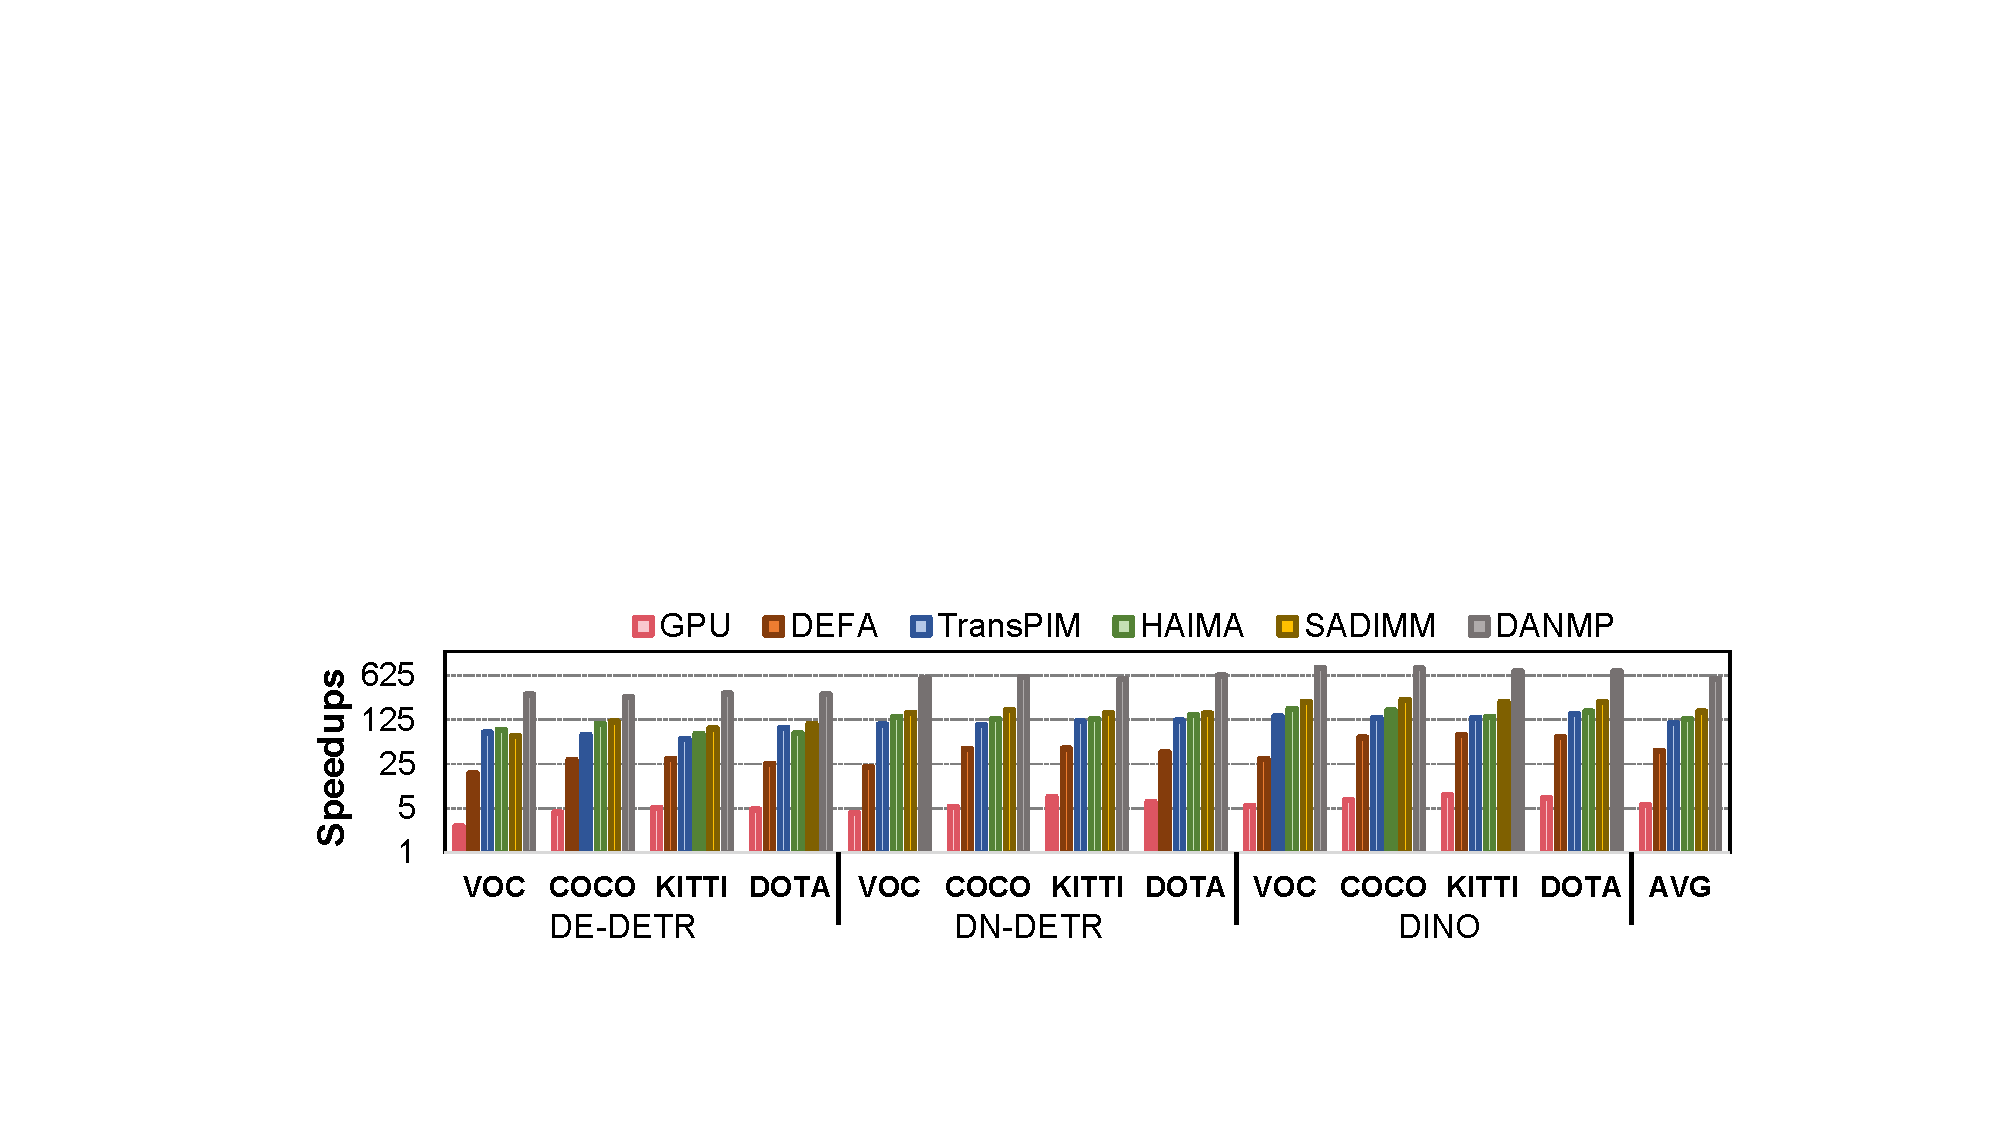
\includegraphics[width=8.3cm]{figures/exp/performance.pdf}
\vspace{-1em}
\caption{Speedup of \textit{DANMP} compared with GPU, {DEFA}, TransPIM, HAIMA, and SADIMM (normalized to CPU)}
\label{performance}
\vspace{-2em}
\end{figure}

\subsection{Overall Performance}
\label{overall_p}
Figure~\ref{performance} presents the performance of \textit{DANMP} against CPU, GPU, DEFA, TransPIM, HAIMA, and SADIMM.

{\bf Comparison with CPU and GPU.} CPUs and GPUs are the mainstream platforms for accelerating Deformable DETR inference. Across all evaluated datasets and models, \textit{DANMP} delivers an average speedup of 557.31$\times$ over the CPU baseline and 97.43$\times$ over the GPU. This remarkable performance gain stems from three key factors: (1) \textit{DANMP} is specifically optimized—both in hardware and software—for MSDAttn, making it far more suitable for DETR workloads than general-purpose architectures.
(2) Its near-memory architecture minimizes costly host-to-memory data transfers, which typically become a bottleneck in memory-intensive tasks.
(3) By integrating processing units directly at the bank level, \textit{DANMP} unleashes the full potential of DRAM bandwidth, which is essential for the heavy memory access patterns of MSDAttn. 



{{\bf Comparison with DEFA.} DEFA is the SOTA ASIC-based accelerator for MSDAttn. Compared to DEFA, DANMP achieves an average speedup of 13.74$\times$, primarily due to two architectural advantages. First, DANMP leverages near-memory parallelism by integrating processing elements directly adjacent to DRAM banks. This design eliminates frequent off-chip memory transfers and enables high-throughput, low-latency data access. Second, DANMP adopts a Clustering-and-Packing (CAP) algorithm that identifies and groups redundant queries across consecutive frames, significantly reducing memory access overhead in streaming workloads.} 


{\bf Comparison with TransPIM and HAIMA.} TransPIM and HAIMA are state-of-the-art accelerators optimized for standard self-attention. Nevertheless, \textit{DANMP} surpasses them by 5.17$\times$ and 4.26$\times$ on average, respectively. The reasons for this advantage include: (1) TransPIM and HAIMA target dense matrix multiplications typical of self-attention, whereas MSDAttn involves irregular and sparse operations that GEMM units handle poorly. \textit{DANMP} addresses this with specialized PEs that execute MSGS directly in memory. (2) Their dataflows and schedulers are designed for regular patterns, making them less effective for MSDAttn’s complexity. In contrast, \textit{DANMP} introduces a custom NMP dataflow tailored to MSDAttn's irregular behavior, improving runtime efficiency. (3) Unlike MSDAttn, self-attention workloads are regular, so prior accelerators overlook dynamic load balancing. In MSGS, severe load imbalance can leave some banks with minimal data for their PEs, causing idle cycles after local computations. \textit{DANMP} addresses this with non-uniform hardware integration, aligning resources with workload irregularity to reduce PE idling. Moreover, relocating cold data within a bank-group requires only a read from the source bank, significantly lowering overhead compared to cross-bank transfers. {While DANMP employs fewer PEs than TransPIM, its throughput is higher because both architectures perform the same computation, making latency the key factor. The latency is dominated by the most loaded bank–PE pair. DANMP’s query grouping greatly improves data reuse among nearby queries, reducing redundant data movement and PE idle time. As a result, DANMP achieves lower execution latency for the same workload, delivering higher effective throughput despite using fewer PEs.}


\begin{figure}[t]
\centering
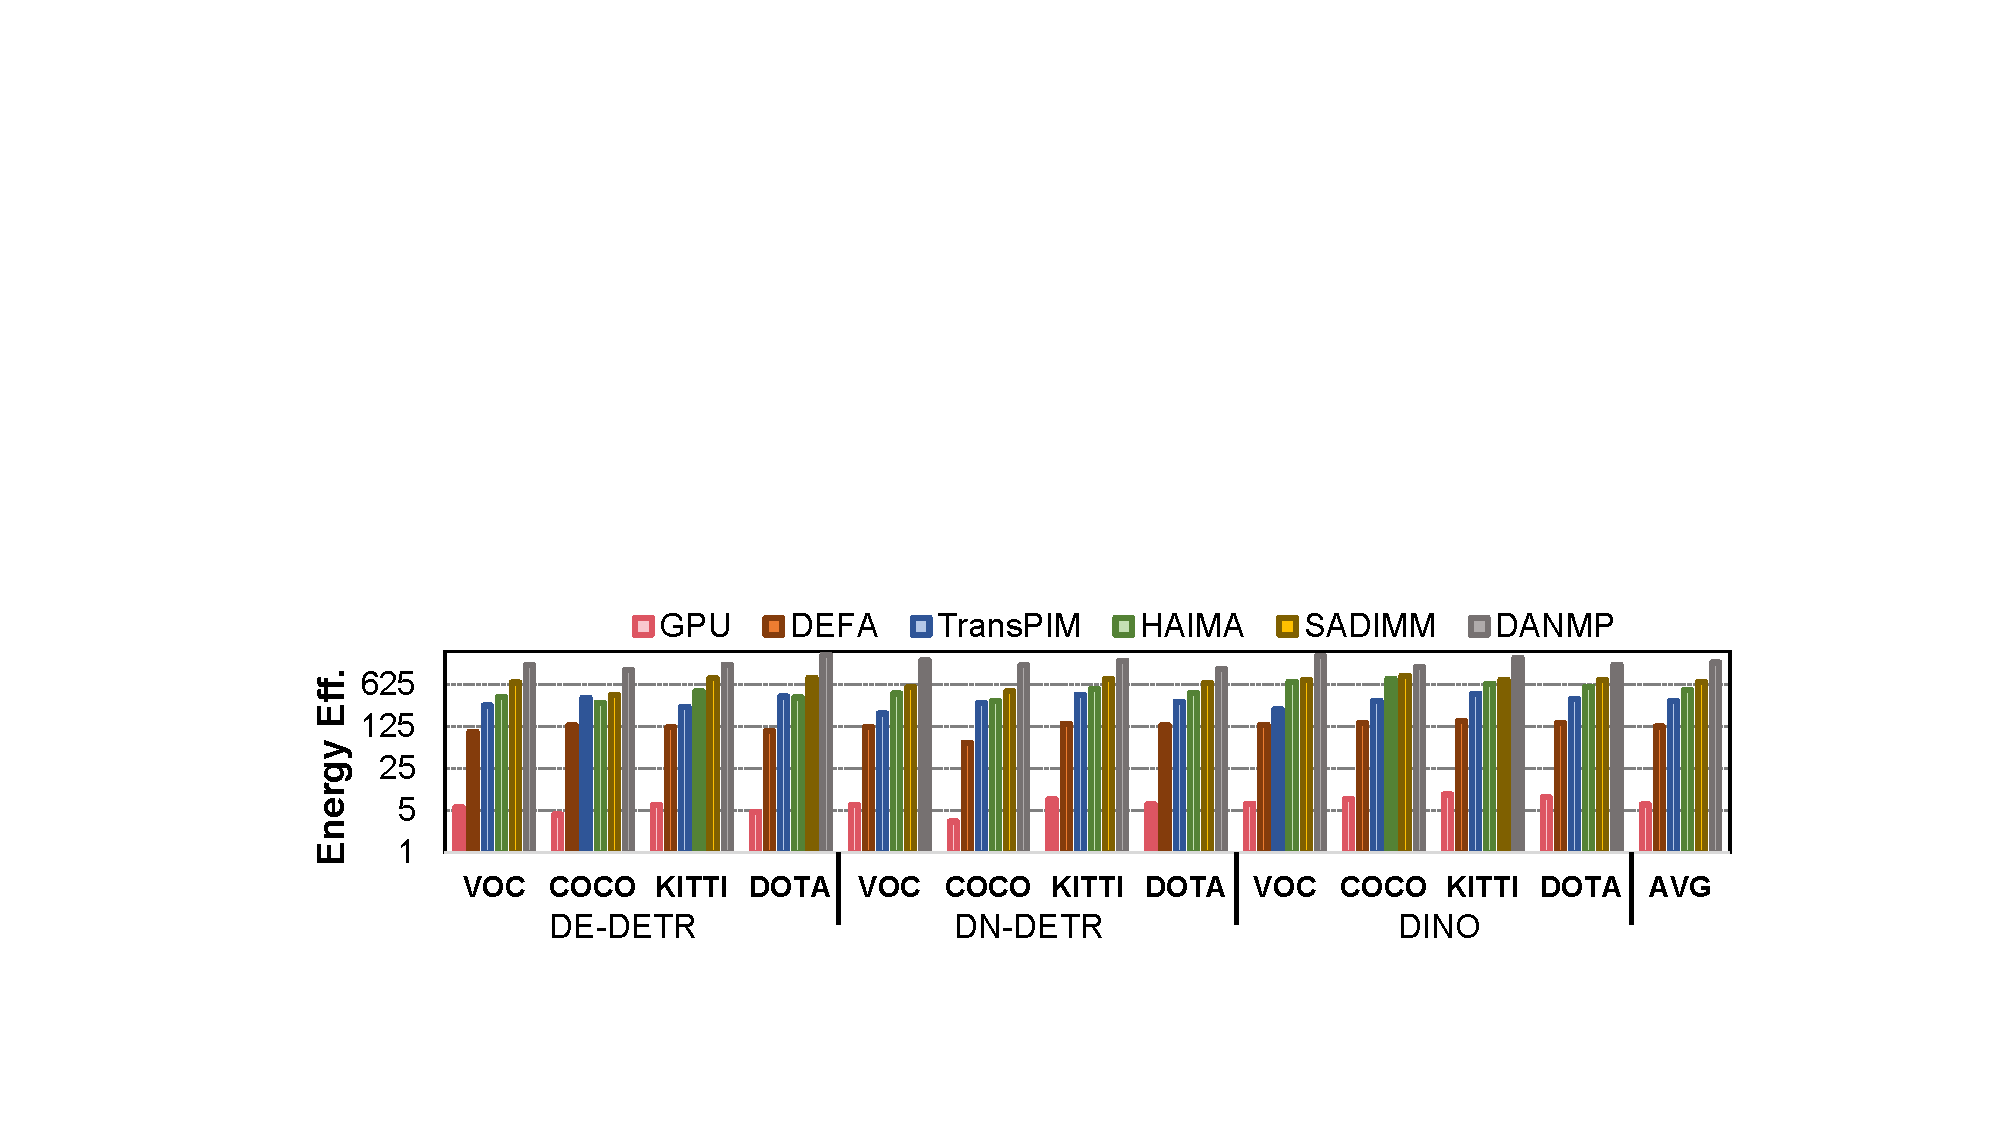
\includegraphics[width=8.3cm]{figures/exp/energy.pdf}
\vspace{-1em}
\caption{Energy efficiency of \textit{DANMP} compared with GPU, {DEFA}, TransPIM, HAIMA, and SADIMM}
\label{energy}
\vspace{-1em}
\end{figure}

{\bf Comparison with SADIMM.} Compared to SADIMM, a leading sparse-attention accelerator, \textit{DANMP} achieves a 3.43$\times$ average speedup. The improvements arise from several innovations: (1) While both adopt efficient memory-side execution, \textit{DANMP} offers a dataflow better suited for MSDAttn. (2) SADIMM introduces a dimension-wise data partitioning strategy to balance load across PEs. However, this method proves insufficient for MSDAttn’s more irregular computation, often resulting in idle compute resources. \textit{DANMP} addresses this through its irregular hardware mapping, aligning hot (cold) entries to bank-level (bank-group level) PEs to ensure balanced execution. (3) SADIMM enhances reuse through diagonal locality in sparse attention~\cite{asadi2024}. Unfortunately, MSDAttn lacks such regularity. \textit{DANMP} compensates by applying the Clustering-and-Packing (CAP) algorithm, which groups queries with shared sub-targets to boost both spatial and temporal data reuse.



{\bf Energy Efficiency Comparison.} Figure~\ref{energy} shows energy efficiency results. {Compared to CPU, GPU, and DEFA platforms, \textit{DANMP} achieves 1437.82$\times$, 227.21$\times$, and 11.63$\times$ improvements, respectively.} {
For completeness, DRAM refresh, DIMM I/O termination, and NMP instruction decoding overheads are also included in the revised estimation.
Their combined contribution accounts for less than 8\% of total system energy, leading to an adjusted overall efficiency of 208.47× over GPU baseline.
} {Compared to the GPU, DANMP achieves a higher improvement in energy efficiency than in performance. This disparity stems from DANMP’s ability to avoid costly off-chip memory accesses, the dominant source of energy consumption. In contrast, GPUs suffer from substantial energy overhead due to frequent data movement and always-on compute resources.} Relative to other NMP accelerators, \textit{DANMP} achieves 4.41$\times$, 2.85$\times$, and 2.37$\times$ better energy efficiency than TransPIM, HAIMA, and SADIMM, respectively. These gains can be attributed to: (1) \textit{DANMP}’s non-uniform integration strategy ensures that near-bank PEs are only deployed where needed, reducing energy waste from idle units. In contrast, platforms with uniform integration must reallocate tasks through costly cross-bank communication. (2) The clustering-and-packing algorithm also significantly increases data reuse, reducing redundant memory accesses and thereby lowering energy per operation.

\begin{figure}[t]
\centering
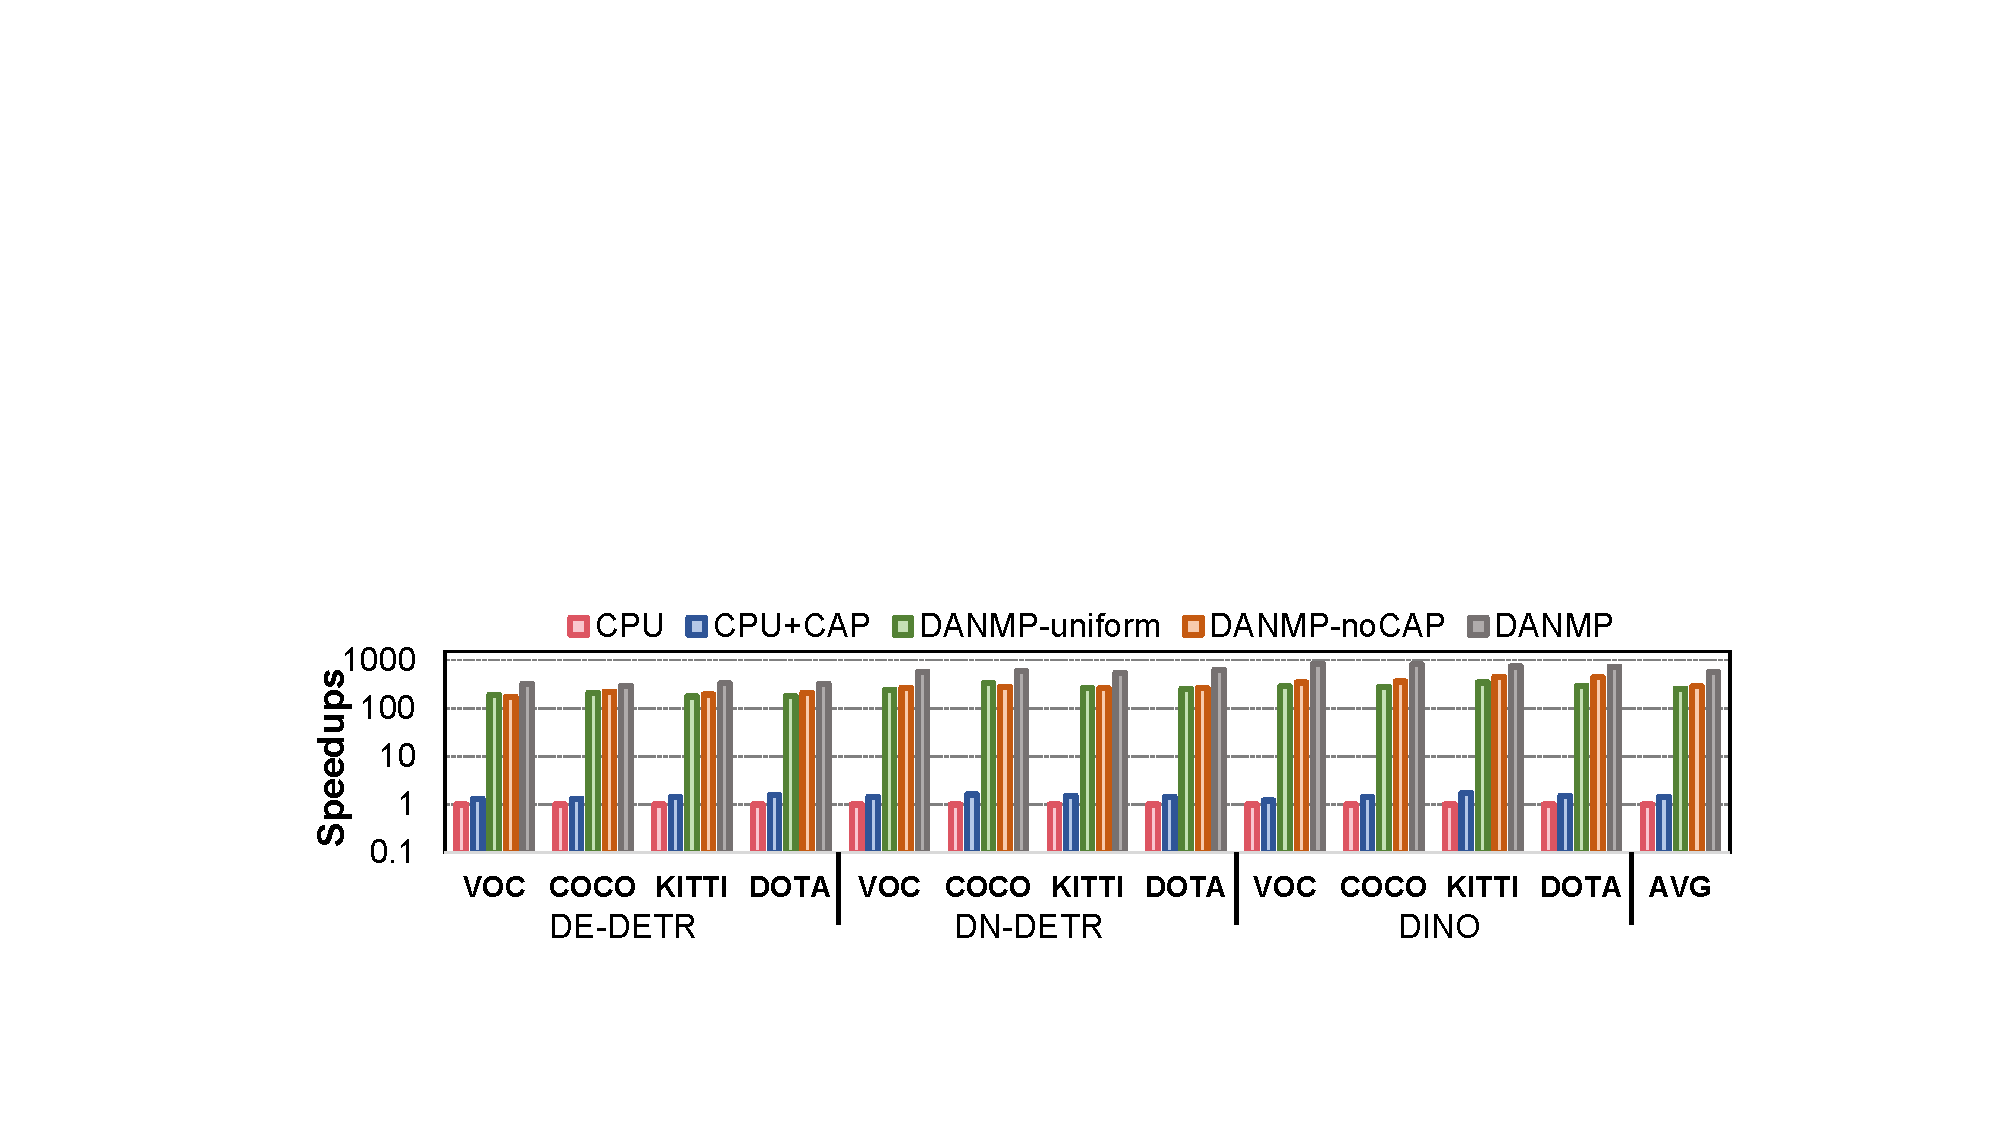
\includegraphics[width=8.3cm]{figures/exp/softonly.pdf}
\vspace{-1em}
\caption{Performance comparison of extra configurations}
\label{softonly}
%\vspace{-2em}
\end{figure}

\subsection{Hardware and Software Efficiency}
\label{hard_soft}
To better understand the individual contributions of \textit{DANMP}'s hardware and software components, we conducted experiments across three supplementary platforms: (1) CPU+CAP, where the CAP algorithm is applied during DETR query inference on the CPU to improve data locality; (2) DANMP-uniform, where identical bank-level PEs are integrated into all banks in DANMP; and (3) DANMP-noCAP, which runs \textit{DANMP} without CAP to isolate its software impact. {The results are shown in Figure~\ref{softonly}.}

{\bf Software Effectiveness.} {Compared to the CPU baseline, integrating CAP yields a 1.45× speedup, demonstrating its effectiveness. Although it introduces clustering and packing overhead, CAP significantly improves data reuse and reduces redundant memory accesses.} This gain arises from two key benefits. First, CAP organizes queries sharing common sub-targets, avoiding repeated computations on overlapping regions. Second, by grouping spatially correlated queries, CAP improves temporal locality, minimizing redundant memory accesses and mitigating random access overhead. These findings support the insight that combining multiple ML strategies is often essential for improving system efficiency in practice.

{\bf Hardware Effectiveness.} Compared to DANMP-uniform, DANMP achieves a 2.21× performance boost. Although CAP improves data reuse in DANMP-uniform, its uniform hardware configuration cannot adapt to the irregular access patterns of MSDAttn, causing significant PE underutilization. To avoid idling, data must be transferred from other banks via the MC, which is far less efficient than local bank-group reads. Moreover, DANMP-uniform provides no more compute resources than \textit{DANMP}, as \textit{DANMP} reallocates some PEs to the bank-group level for better load balancing. Even without CAP optimization, DANMP-noCAP still surpasses the CPU baseline by a large margin, achieving a 283.63× speedup. This improvement mainly results from the NMP-based architecture, which minimizes off-chip transfers, and the near-bank computing scheme that significantly increases available bandwidth. Although omitting CAP introduces some bandwidth inefficiencies, \textit{DANMP} still maintains a substantial advantage, underscoring the potential of NMP-based architectures for specialized DETR acceleration.



\begin{figure}[t]
\centering
\subfloat[]{
\begin{minipage}[t]{0.489\linewidth}
\centering
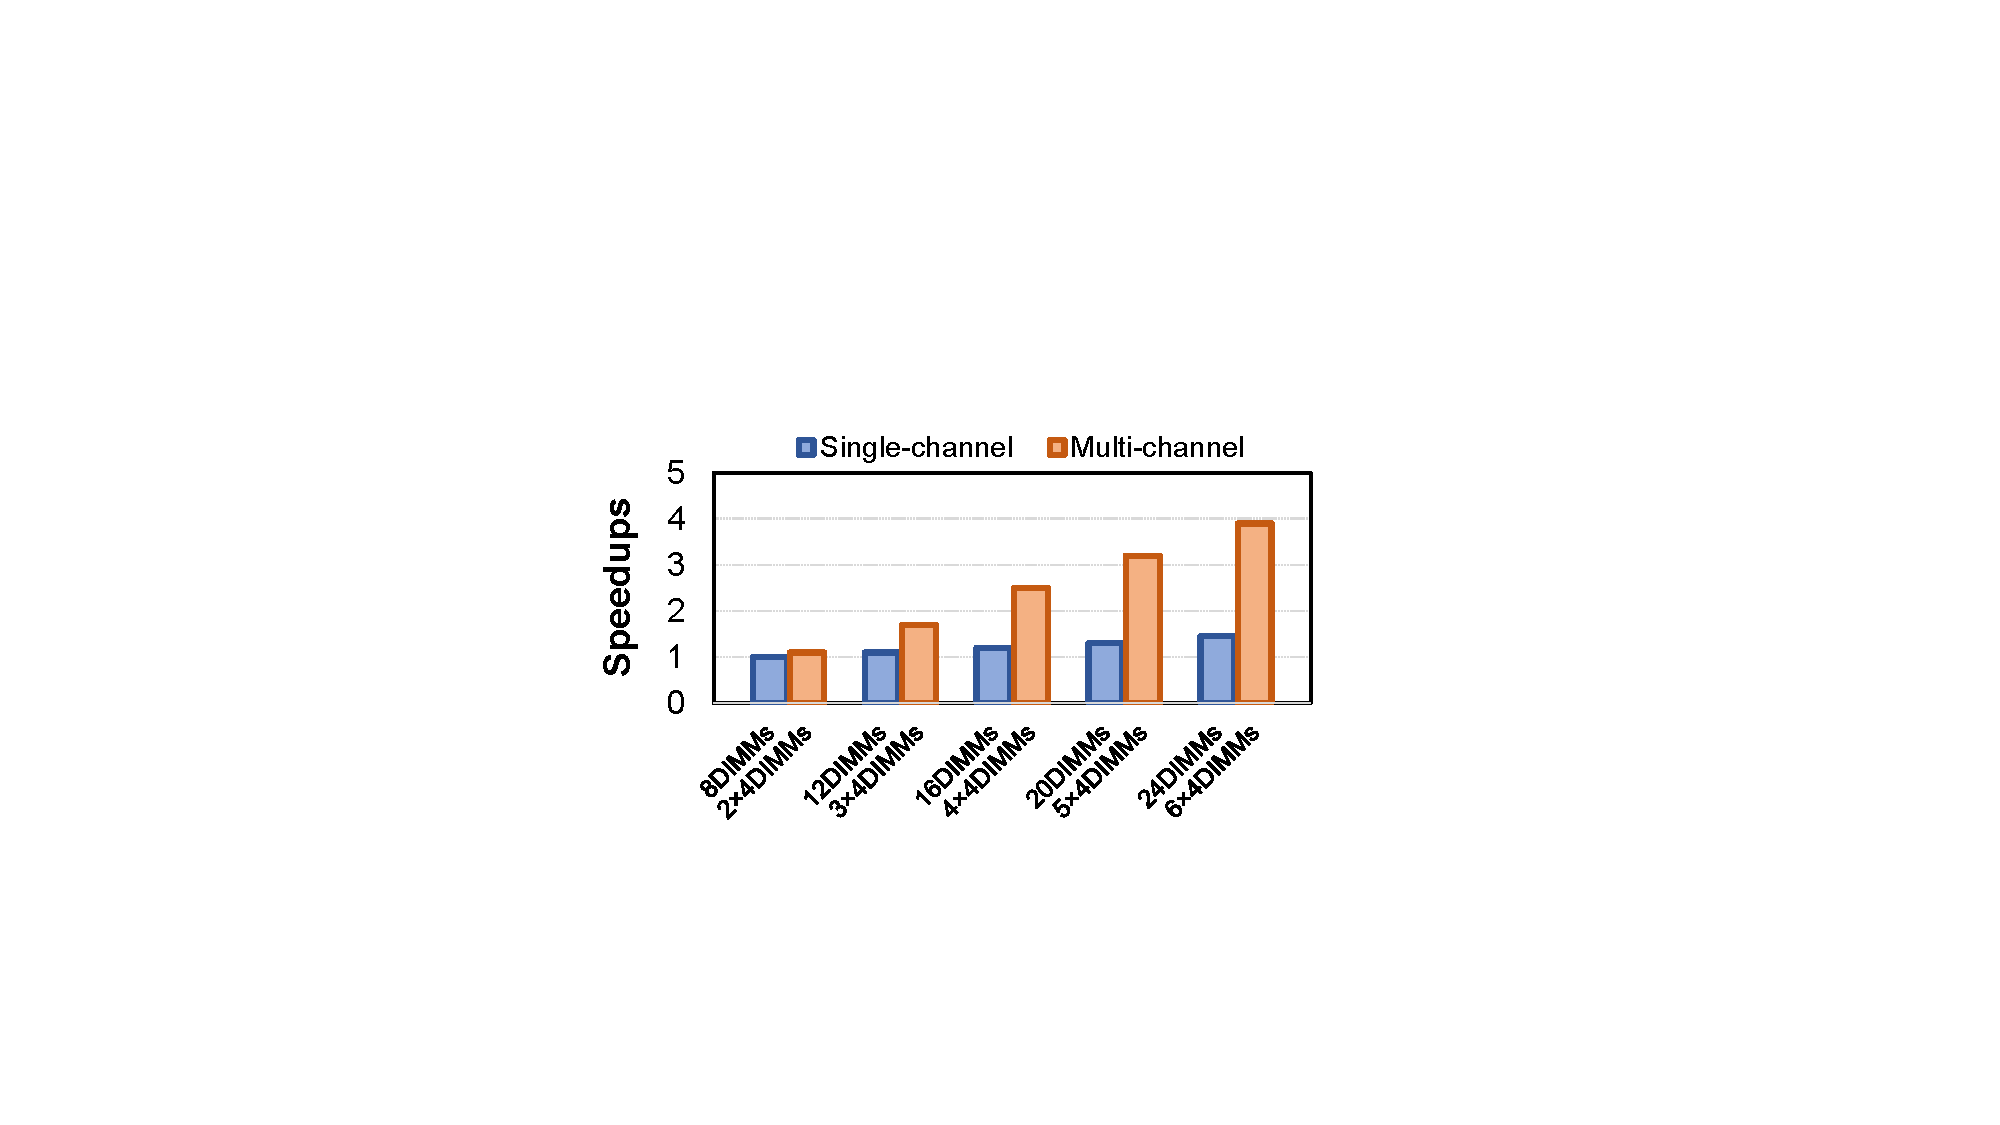
\includegraphics[width=1.5in]{figures/exp/dimm.pdf}
\end{minipage}
}%
\subfloat[]{
\begin{minipage}[t]{0.489\linewidth}
\centering
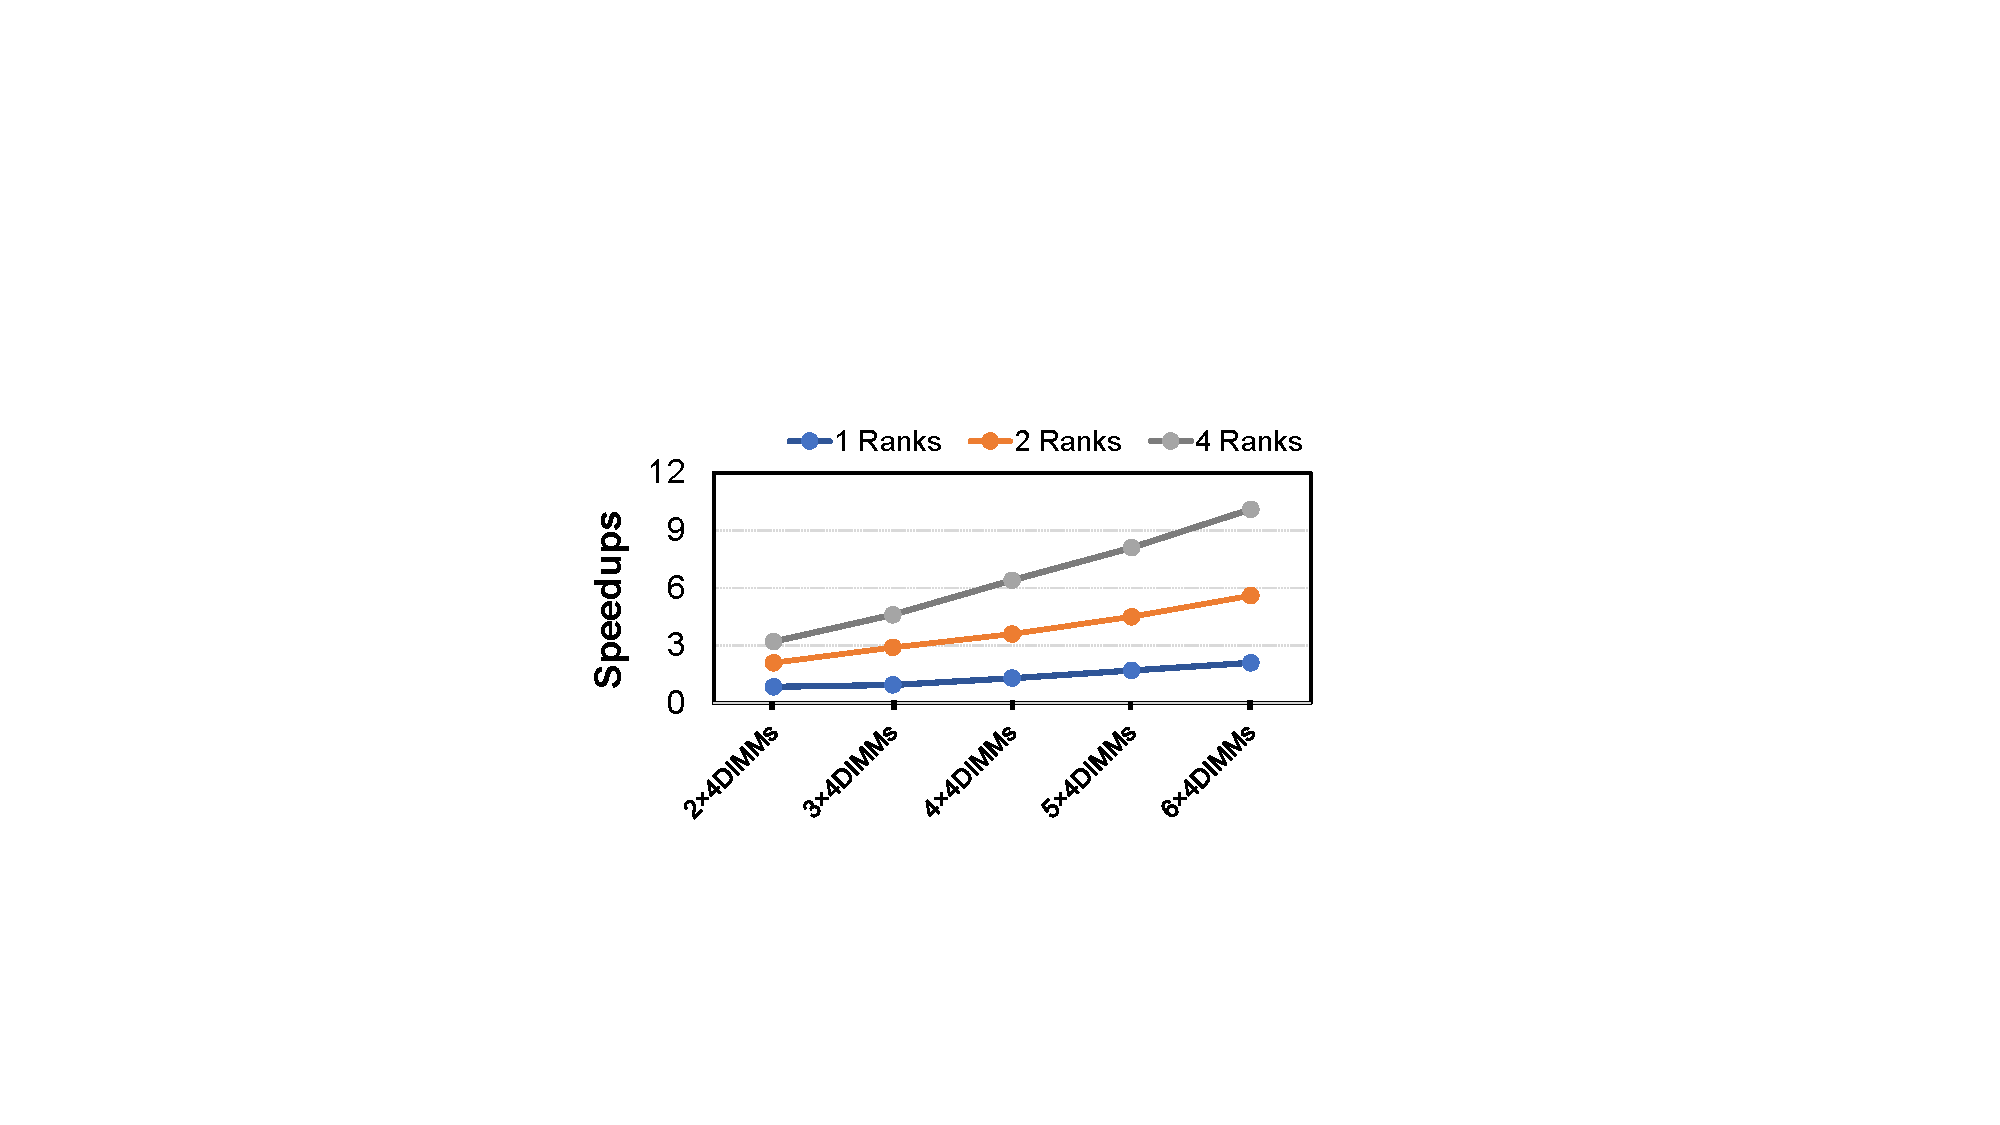
\includegraphics[width=1.5in]{figures/exp/rank.pdf}
\end{minipage}
}%
\centering
\vspace{-1em}
\caption{(a) Scalability of \textit{DANMP} on DE-DETR as the number of DIMMs increases, and (b) Performance of \textit{DANMP} with different number of ranks}
\vspace{-1em}
\label{hard_scalability}
%\vspace{-1em}
\end{figure}

\subsection{Scalability}
\label{scala_exp}
{\bf Impact of DIMM and Rank Configuration.} Figure~\ref{hard_scalability}(a) shows \textit{DANMP} performance scaling on MSDAttn workloads {under varying DIMM and memory channel counts.} Results reveal that simply increasing DIMMs on a single memory channel yields limited improvement. Although more DIMMs provide higher internal bandwidth, control signals remain constrained by the single channel, making it the bottleneck. In contrast, adding DIMMs across multiple channels significantly boosts throughput by removing this constraint and enabling parallel C/A paths. Figure~\ref{hard_scalability}(b) further examines performance changes with rank count per DIMM. While adding ranks enhances bandwidth at the rank level, gains are sublinear due to shared bus connections. Nonetheless, performance improves steadily—for example, a 4-rank configuration achieves a 1.63× speedup over 2 ranks, demonstrating that \textit{DANMP} effectively exploits bandwidth hierarchy across ranks.

\begin{figure}[t]
\centering
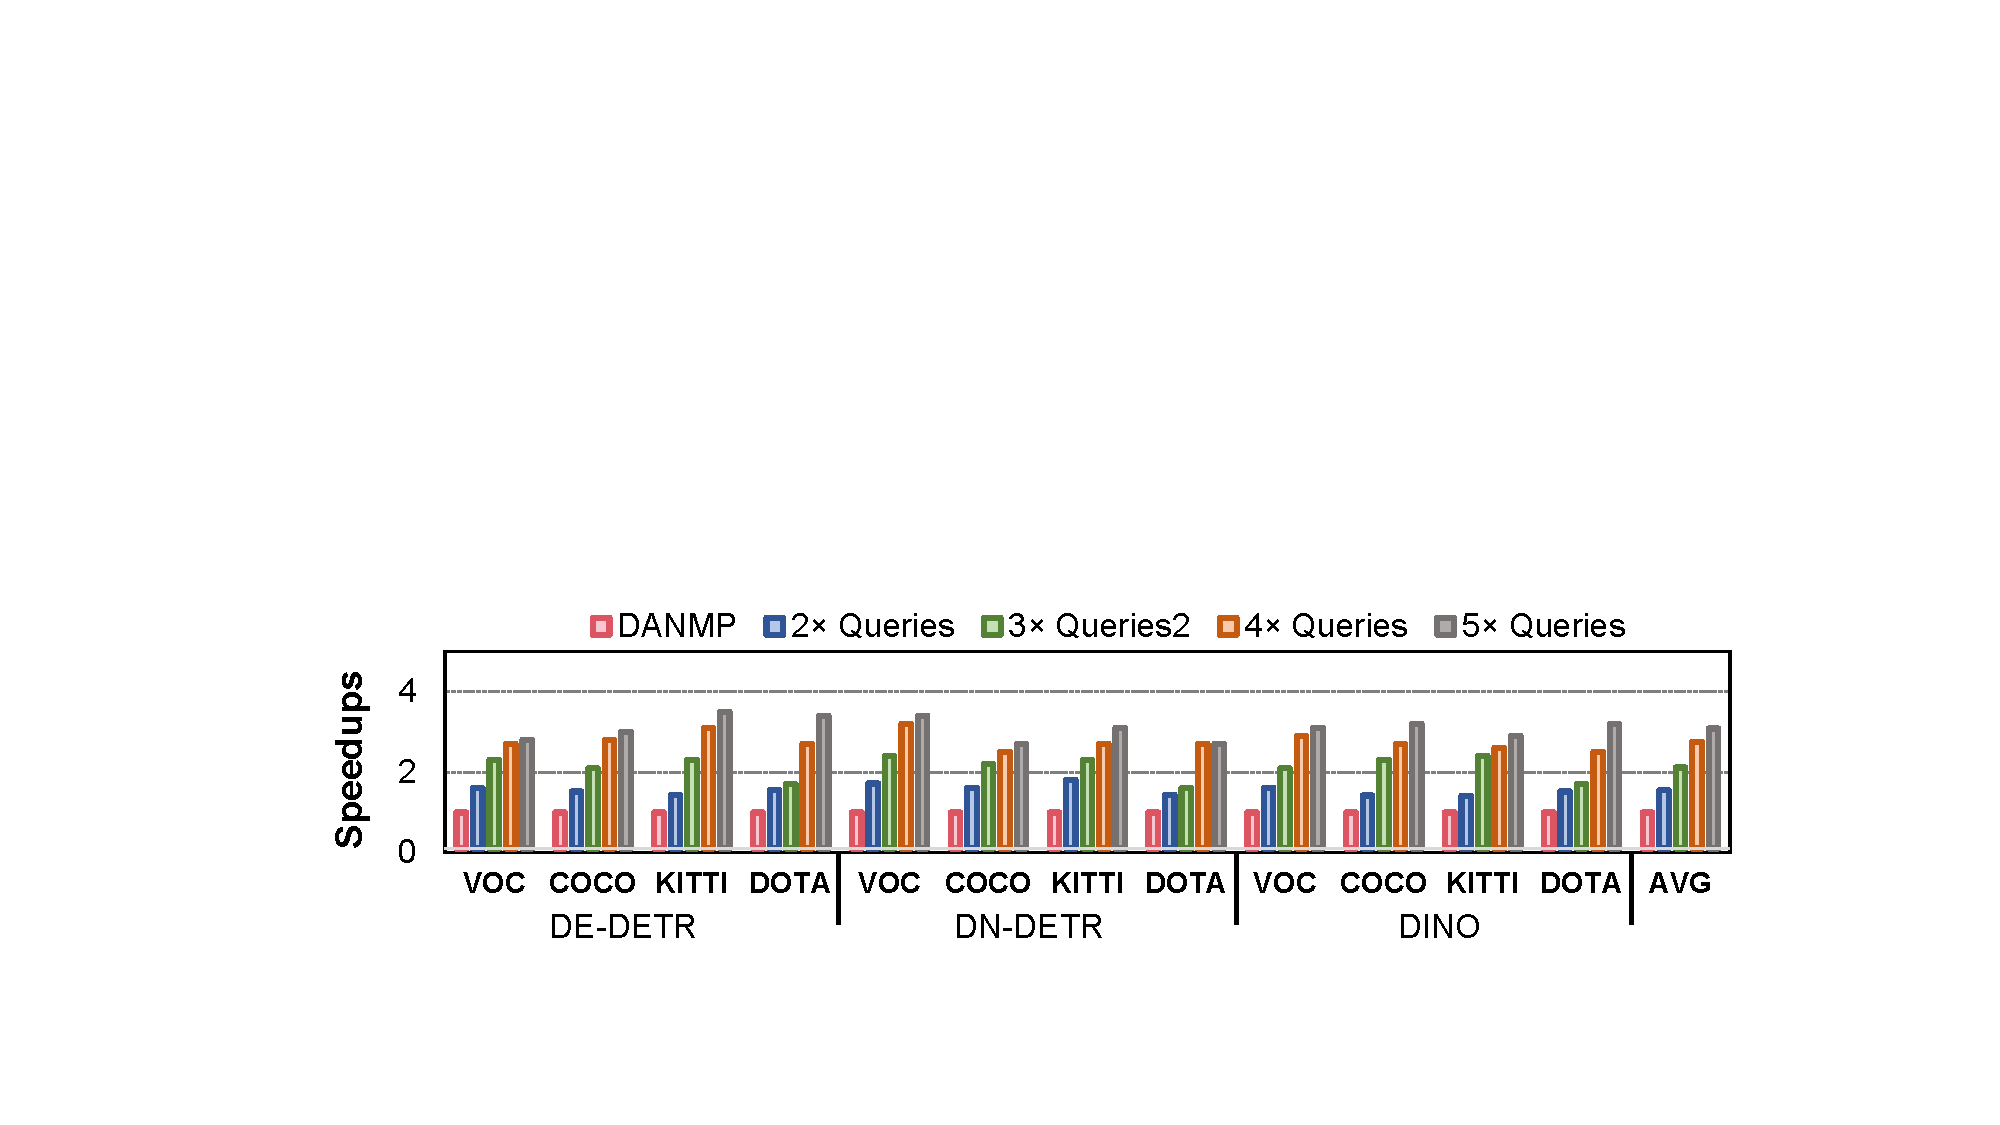
\includegraphics[width=8.3cm]{figures/exp/queries.pdf}
\vspace{-1em}
\caption{The speedups with various number of queries}
\label{query_scala}
%\vspace{-2em}
\end{figure}

{\bf Impact of Query Volume.} We simulate expanded workloads by proportionally increasing the number of queries and feature map dimensions. For instance, the "2× Queries" setup doubles the query and feature map sizes compared to the baseline. As shown in Figure~\ref{query_scala}, \textit{DANMP}'s performance gain over the CPU baseline continues to grow with the number of queries. This trend highlights \textit{DANMP}’s strong scalability in large-scale inference tasks. First, the use of near-memory computing minimizes the off-chip random memory access overhead. This advantage becomes more pronounced as the number of queries increases. Second, the CAP algorithm enhances temporal and spatial data reuse by clustering queries that target overlapping regions. As the number of queries increases, the probability of shared sub-targets rises, leading to even higher reuse efficiency.

{{\bf Impact of CAP Sampling Rate.} Figure~\ref{latency_break}(b) presents the experimental results of the impact of CAP clustering ratio on normalized inference latency. {The x-axis represents cumulative query progress (50, 100, 150, 200, 250, and 300 queries), and the y-axis shows the corresponding latency. The clustering-and-packing overhead is already included. Since it is performed only once for 300 queries, and the latency of a single query is higher than the packing overhead..} Compared to the no-CAP baseline, CAP with various sampling ratios consistently achieves lower latency, demonstrating its effectiveness. The lowest latency is observed when 20\% of the queries are selected for coordinate clustering, as the remaining 80\% benefit from improved data reuse enabled by CAP. A smaller ratio, such as 10\%, is not chosen because it yields limited benefits on feature maps with only 100 queries. We set 20\% as the default configuration because it achieves the best trade-off between clustering effectiveness and minimal inference latency.}

\begin{figure}[t]
\centering
\subfloat[]{
\begin{minipage}[t]{0.489\linewidth}
\centering
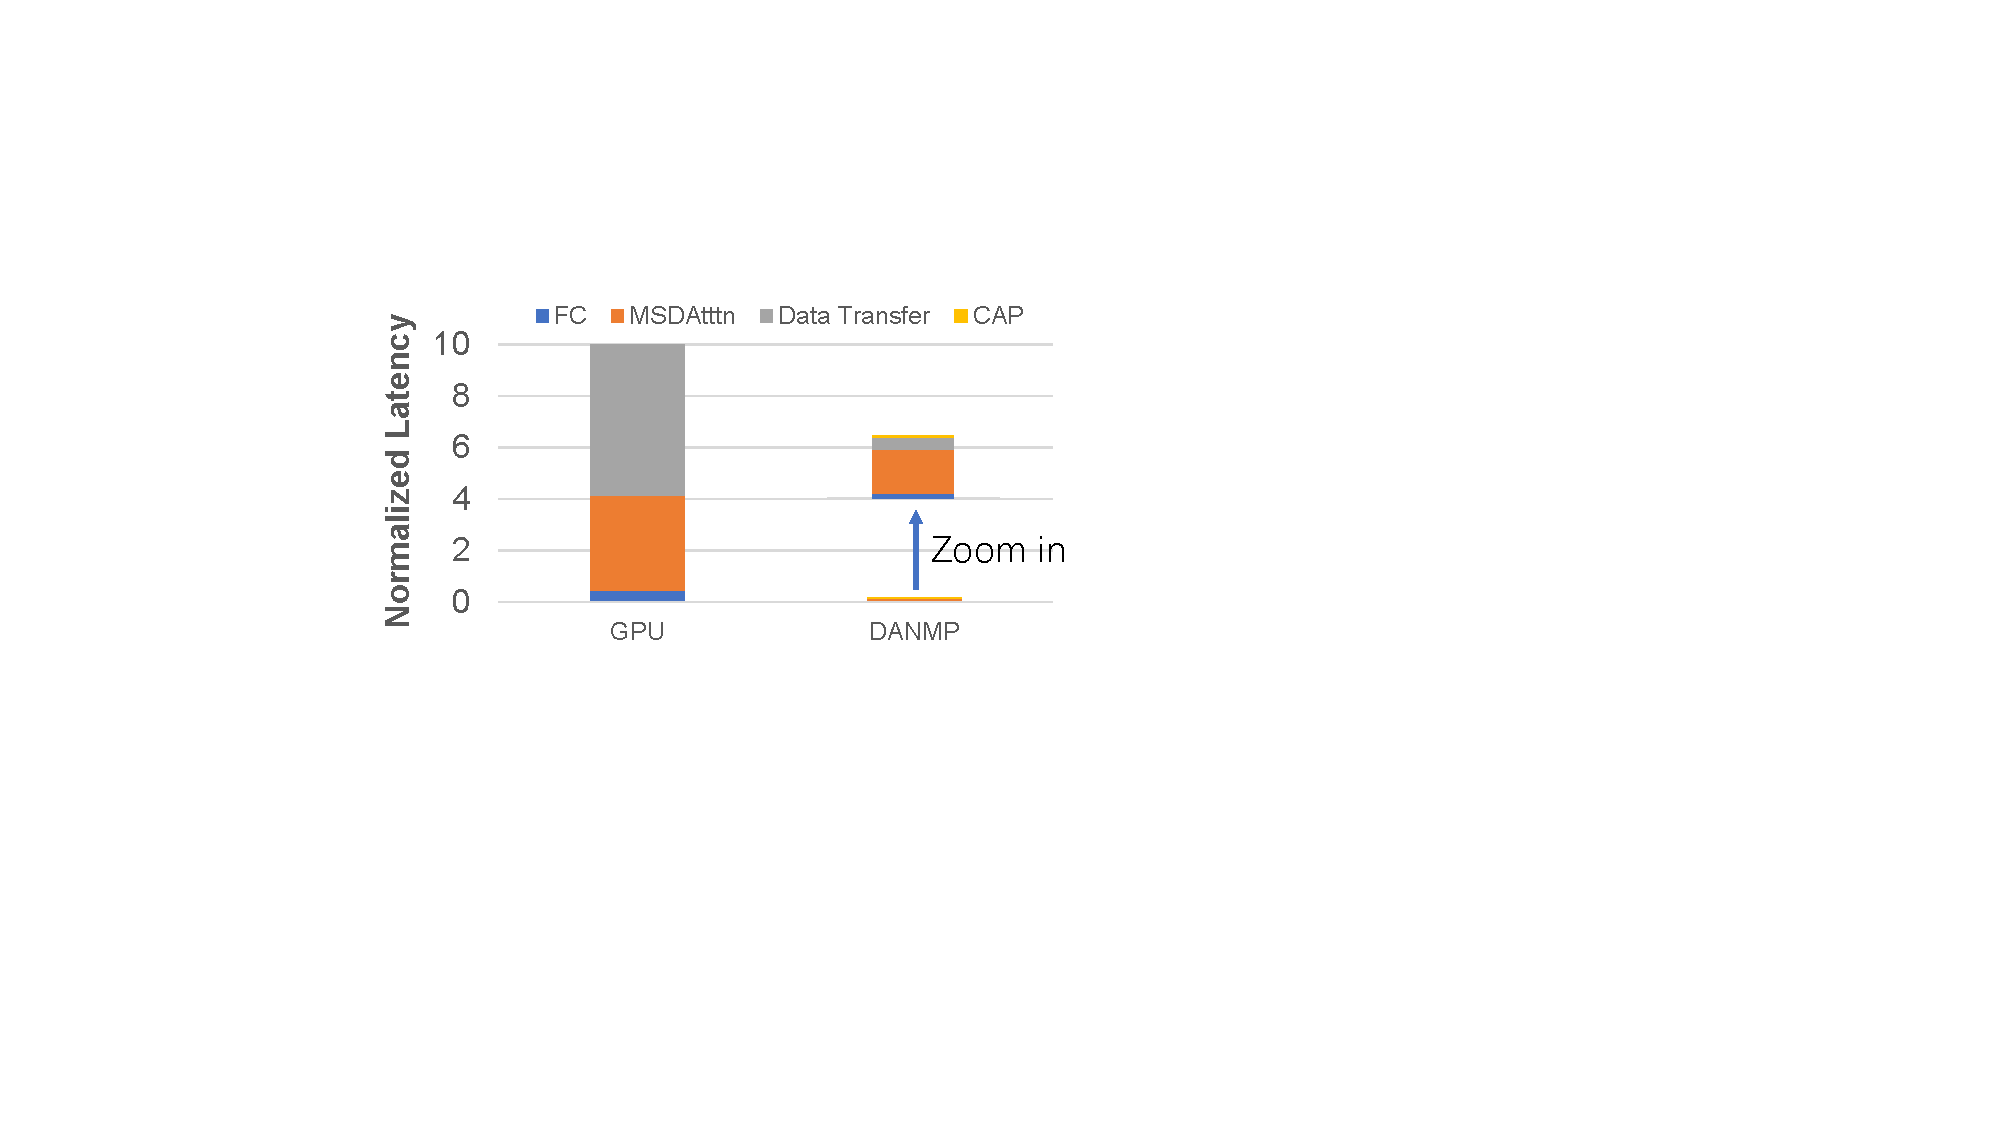
\includegraphics[width=1.5in]{figures/exp/latency_break.pdf}
\end{minipage}
}%
\subfloat[]{
\begin{minipage}[t]{0.489\linewidth}
\centering
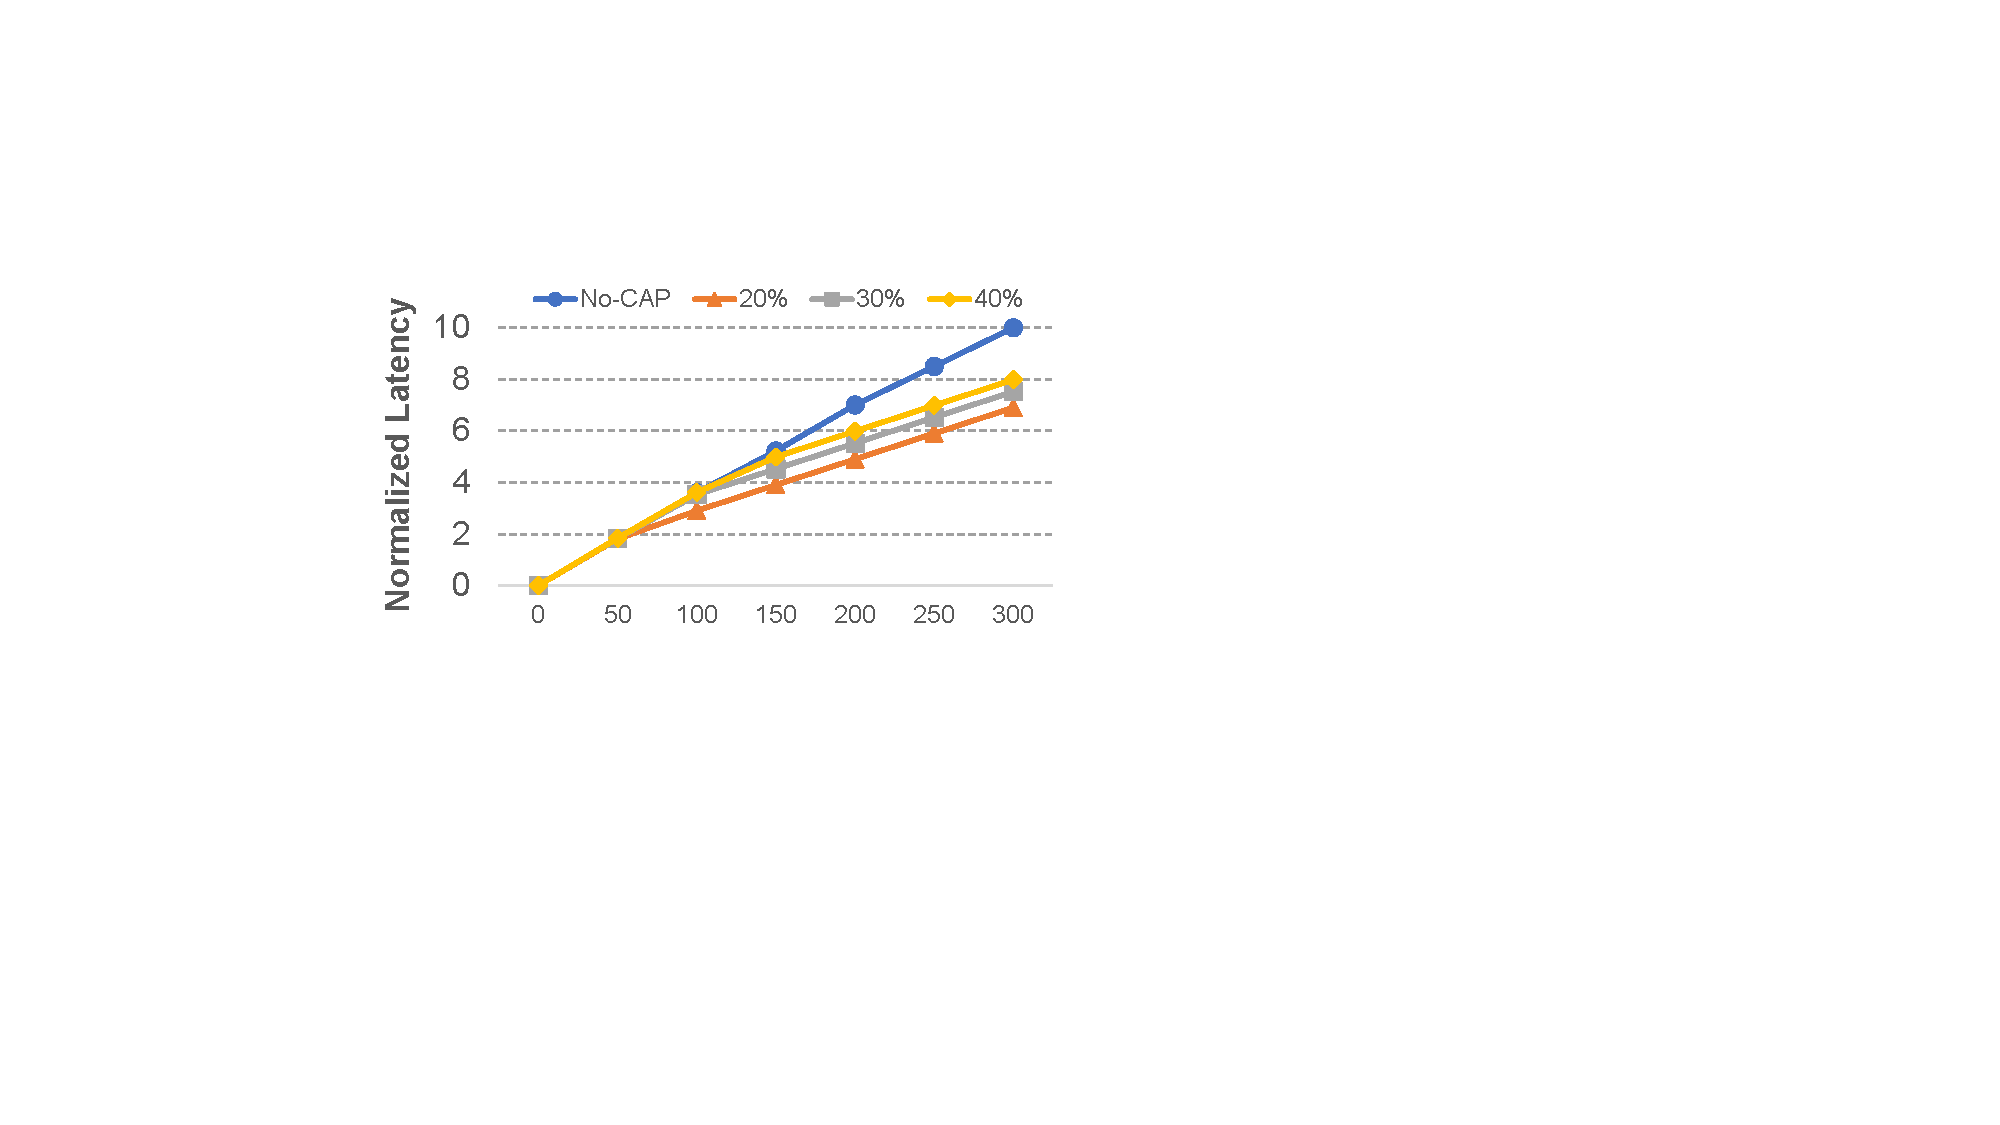
\includegraphics[width=1.5in]{figures/exp/sample.pdf}
\end{minipage}
}%
\centering
\vspace{-0.5em}
\caption{(a) Latency breakdown of a DE-DETR transformer block (COCO, 100 queries per FMap, batch size 8), and (b) Impact of CAP clustering ratio on normalized inference latency (CPU, 300 queries per FMap, batch size 8)}
\vspace{-1em}
\label{latency_break}
%\vspace{-1em}
\end{figure}


\subsection{{Latency/}Energy/Area Breakdown}
\label{lea_break}
{\bf Latency Breakdown.} Figure~\ref{latency_break}(a) shows the latency breakdown of a transformer block in DE-DETR on the COCO dataset, with 100 queries per feature map and a batch size of 8. On GPU, MSDAttn accounts for 36.4\% of total latency, while data movement dominates with 59.2\%, reflecting the low cache hit rate in Figure~\ref{case1}(b). The FC layer contributes less than 5\%, as its regular access pattern overlaps effectively with data transfers, consistent with prior studies~\cite{kao2023flat, gilbert2024looptree, lee2024infinigen}. {In \textit{DANMP}, CAP, FC, data movement, and MSDAttn contribute 1.3\%, 8.6\%, 27.4\%, and 62.7\% of latency, respectively, indicating minimal CAP overhead.} Although the FC layer runs on the CPU, its latency remains low due to overlap with data transfers. {Unlike the GPU, where FC execution is delayed by the long MSDAttn stage due to data dependencies, DANMP’s faster NMP-based MSDAttn shortens this dependency chain, resulting in significantly less FC stall time and reducing the overall latency.} Despite being an NMP accelerator, DANMP incurs 27\% data movement overhead, primarily from transferring weight matrices to the CPU.


{\bf Energy/Area Breakdown.} We present the area and power consumption of SADIMM and \textit{DANMP} in Table~\ref{tab:breakdown}. {In 40nm technology, \textit{DANMP} shows a minimal rank PE area per buffer chip of 0.42 $mm^2$, a notable reduction from SADIMM’s 0.73 $mm^2$, mainly because the rank PE in \textit{DANMP} only handles aggregation and omits softmax. \textit{DANMP} exhibits a bank-group PE area per DRAM chip of 0.57 $mm^2$, slightly larger than SADIMM’s 0.39 $mm^2$, since BG-level PEs in \textit{DANMP} share part of the workload originally handled by bank-level PEs. \textit{DANMP} also shows a minimal bank PE area per DRAM chip of 1.03 $mm^2$, a significant reduction from SADIMM’s 2.29 $mm^2$. Furthermore, \textit{DANMP} consumes 259 $mW$, 31.6\% lower than SADIMM’s 335 $mW$.}

\begin{table}[t]
\centering
\tabcolsep=0.05cm
    \caption{Power and area breakdown of \textit{DANMP}}
    \vspace{-1em}
    %\renewcommand\arraystretch{0.8}
    \label{tab:breakdown}
    %\tabcolsep=0.05cm
    \begin{tabular}{|c|c|c|c|c|}  
    \cline{1-5}
    
       {\bf Name} & {\bf Component}& {\bf PE type} & {\bf Area (mm$^2$) } & {\bf Power (mW)}\\
       \hline \hline

       
       \multirow{3}*{SADIMM} & {Rank PEs} & {adder\&soft.} & {0.73} & {82} \\
       \cline{2-5}
       {} & {BG PEs} & {adder} & {0.39} & {37} \\
       \cline{2-5}
       {} & {Banks PEs} & {multiplier} & {2.29} & {216} \\
       \hline
       \multirow{3}*{DANMP} & {Rank PEs} & {MAC Unit} & {0.42} & {51} \\
       \cline{2-5}
       {} & {BG PEs} & {ICU\&BICU} & {0.57} & {71} \\
       \cline{2-5}
       {} & {Bank PEs} & {ICU\&BICU} & {1.03} & {137} \\
       \cline{1-5}
    
\end{tabular}
%\vspace{-1.5em}
\end{table}

\subsection{Discussion}
\label{discussion}

{
{\bf Support Other Applications.} We discuss how \textit{DANMP} benefits other memory-bound workloads. A prime example is graph processing, known for its irregularity: high-degree nodes require heavy computation, while low-degree ones are lightweight. Uniform assignment causes runtime inefficiencies. \textit{DANMP}’s heterogeneous integration addresses this by allocating heavy, high-degree nodes to bank-level PEs and lighter ones to bank-group PEs, enhancing efficiency. Similarly, in databases, frequently accessed fields (e.g., primary keys) can be routed to bank-level PEs, leaving less active fields to bank-group units. While not aiming for a universal accelerator, our insights—such as clustering-based reuse and non-uniform PE integration—can guide future NMP architectures for graph analytics, sparse vision, and other irregular applications.}




\section{Related Works}
{\bf Traditional Attention Accelerators.} Early efforts to accelerate Transformer-based models largely leveraged GPUs due to their high parallel computing capabilities~\cite{Vaswani17, bert18, longformer20, Flashatten2022, zhu2021deformable, Li_2022_CVPR, zhang2023dino, Aken19, RoBERTa2019, Arnab_2021_ICCV}. GPU-focused approaches~\cite{longformer20, Flashatten2022, Zaheer20, Performer2020, Linformer2020, wu2020visual, Zaheer20} aim to reduce memory consumption and computational complexity in attention modules. To further alleviate compute and memory overheads, co-designed accelerators have been developed using FPGAs~\cite{Zhang21, bai2024dac, Li20, Ye2023} and ASICs~\cite{Ham20, Lu21, Qu22, xu2024defa, Qin2023, You2023}. These platforms provide better support for custom scheduling and attention-specific logic. However, their performance remains limited by frequent random memory accesses and the increasing cost of off-chip memory transfers, with bandwidth quickly becoming the system bottleneck~\cite{Xie2021, pim-mmu2024}.

{\bf Near-Memory Attention Acceleration.} Near-memory processing (NMP) architectures offer a promising alternative by enabling in-memory data processing and reducing off-chip traffic. These architectures have shown notable improvements in bandwidth utilization and throughput across memory-intensive workloads such as non-Transformer deep learning~\cite{Gao2017, ReGNN2022, Xu2024, Kal2021, Park2021, Liu2023, Angizi2018}, graph processing~\cite{Talati2022, Dai2022, Zhang2018}, and attention models~\cite{li2022cpsaa, Zhou2022, Ding2023, asadi2024, sadimm2025, Yang20, Kang21, Laguna2021, Zhou2021, sprint2022, Li2023, Sridharan2023, Zheng2023}. While NMP designs excel at minimizing memory access latency, many still suffer from inefficient PE utilization due to workload imbalance and limited data reuse opportunities. These shortcomings result in increased scheduling overhead and suboptimal resource use. To address these issues, our work proposes a heterogeneous NMP design with non-uniform integration of compute units and introduces a collaborative optimization framework between the host and memory modules.


\section{Conclusion}
This paper targets the memory-bound MSDAttn mechanism. As existing NMP accelerators struggle with utilization and efficiency, we propose \textit{DANMP}, a hardware–software co-designed solution. \textit{DANMP} employs selective PE integration, placing compute units only in designated banks to match MSDAttn’s irregularity and reduce cross-bank communication. In software, the CAP method ensures efficient execution via a tailored dataflow. Experiments demonstrate that \textit{DANMP} significantly outperforms state-of-the-art NMP accelerators in both performance and energy efficiency.

%%
%% The next two lines define the bibliography style to be used, and
%% the bibliography file.
\bibliographystyle{ACM-Reference-Format}
\bibliography{sample-base}




\end{document}
\endinput
%%
%% End of file `sample-sigconf-authordraft.tex'.
S